% Options for packages loaded elsewhere
% Options for packages loaded elsewhere
\PassOptionsToPackage{unicode}{hyperref}
\PassOptionsToPackage{hyphens}{url}
\PassOptionsToPackage{dvipsnames,svgnames,x11names}{xcolor}
%
\documentclass[
  nonatbib,
  authoryear,
  preprint]{elsarticle}
\usepackage{xcolor}
\usepackage{amsmath,amssymb}
\setcounter{secnumdepth}{5}
\usepackage{iftex}
\ifPDFTeX
  \usepackage[T1]{fontenc}
  \usepackage[utf8]{inputenc}
  \usepackage{textcomp} % provide euro and other symbols
\else % if luatex or xetex
  \usepackage{unicode-math} % this also loads fontspec
  \defaultfontfeatures{Scale=MatchLowercase}
  \defaultfontfeatures[\rmfamily]{Ligatures=TeX,Scale=1}
\fi
\usepackage{lmodern}
\ifPDFTeX\else
  % xetex/luatex font selection
\fi
% Use upquote if available, for straight quotes in verbatim environments
\IfFileExists{upquote.sty}{\usepackage{upquote}}{}
\IfFileExists{microtype.sty}{% use microtype if available
  \usepackage[]{microtype}
  \UseMicrotypeSet[protrusion]{basicmath} % disable protrusion for tt fonts
}{}
\makeatletter
\@ifundefined{KOMAClassName}{% if non-KOMA class
  \IfFileExists{parskip.sty}{%
    \usepackage{parskip}
  }{% else
    \setlength{\parindent}{0pt}
    \setlength{\parskip}{6pt plus 2pt minus 1pt}}
}{% if KOMA class
  \KOMAoptions{parskip=half}}
\makeatother
% Make \paragraph and \subparagraph free-standing
\makeatletter
\ifx\paragraph\undefined\else
  \let\oldparagraph\paragraph
  \renewcommand{\paragraph}{
    \@ifstar
      \xxxParagraphStar
      \xxxParagraphNoStar
  }
  \newcommand{\xxxParagraphStar}[1]{\oldparagraph*{#1}\mbox{}}
  \newcommand{\xxxParagraphNoStar}[1]{\oldparagraph{#1}\mbox{}}
\fi
\ifx\subparagraph\undefined\else
  \let\oldsubparagraph\subparagraph
  \renewcommand{\subparagraph}{
    \@ifstar
      \xxxSubParagraphStar
      \xxxSubParagraphNoStar
  }
  \newcommand{\xxxSubParagraphStar}[1]{\oldsubparagraph*{#1}\mbox{}}
  \newcommand{\xxxSubParagraphNoStar}[1]{\oldsubparagraph{#1}\mbox{}}
\fi
\makeatother


\usepackage{longtable,booktabs,array}
\usepackage{calc} % for calculating minipage widths
% Correct order of tables after \paragraph or \subparagraph
\usepackage{etoolbox}
\makeatletter
\patchcmd\longtable{\par}{\if@noskipsec\mbox{}\fi\par}{}{}
\makeatother
% Allow footnotes in longtable head/foot
\IfFileExists{footnotehyper.sty}{\usepackage{footnotehyper}}{\usepackage{footnote}}
\makesavenoteenv{longtable}
\usepackage{graphicx}
\makeatletter
\newsavebox\pandoc@box
\newcommand*\pandocbounded[1]{% scales image to fit in text height/width
  \sbox\pandoc@box{#1}%
  \Gscale@div\@tempa{\textheight}{\dimexpr\ht\pandoc@box+\dp\pandoc@box\relax}%
  \Gscale@div\@tempb{\linewidth}{\wd\pandoc@box}%
  \ifdim\@tempb\p@<\@tempa\p@\let\@tempa\@tempb\fi% select the smaller of both
  \ifdim\@tempa\p@<\p@\scalebox{\@tempa}{\usebox\pandoc@box}%
  \else\usebox{\pandoc@box}%
  \fi%
}
% Set default figure placement to htbp
\def\fps@figure{htbp}
\makeatother


% definitions for citeproc citations
\NewDocumentCommand\citeproctext{}{}
\NewDocumentCommand\citeproc{mm}{%
  \begingroup\def\citeproctext{#2}\cite{#1}\endgroup}
\makeatletter
 % allow citations to break across lines
 \let\@cite@ofmt\@firstofone
 % avoid brackets around text for \cite:
 \def\@biblabel#1{}
 \def\@cite#1#2{{#1\if@tempswa , #2\fi}}
\makeatother
\newlength{\cslhangindent}
\setlength{\cslhangindent}{1.5em}
\newlength{\csllabelwidth}
\setlength{\csllabelwidth}{3em}
\newenvironment{CSLReferences}[2] % #1 hanging-indent, #2 entry-spacing
 {\begin{list}{}{%
  \setlength{\itemindent}{0pt}
  \setlength{\leftmargin}{0pt}
  \setlength{\parsep}{0pt}
  % turn on hanging indent if param 1 is 1
  \ifodd #1
   \setlength{\leftmargin}{\cslhangindent}
   \setlength{\itemindent}{-1\cslhangindent}
  \fi
  % set entry spacing
  \setlength{\itemsep}{#2\baselineskip}}}
 {\end{list}}
\usepackage{calc}
\newcommand{\CSLBlock}[1]{\hfill\break\parbox[t]{\linewidth}{\strut\ignorespaces#1\strut}}
\newcommand{\CSLLeftMargin}[1]{\parbox[t]{\csllabelwidth}{\strut#1\strut}}
\newcommand{\CSLRightInline}[1]{\parbox[t]{\linewidth - \csllabelwidth}{\strut#1\strut}}
\newcommand{\CSLIndent}[1]{\hspace{\cslhangindent}#1}



\setlength{\emergencystretch}{3em} % prevent overfull lines

\providecommand{\tightlist}{%
  \setlength{\itemsep}{0pt}\setlength{\parskip}{0pt}}



 


\usepackage{booktabs}
\usepackage{longtable}
\usepackage{array}
\usepackage{multirow}
\usepackage{wrapfig}
\usepackage{float}
\usepackage{colortbl}
\usepackage{pdflscape}
\usepackage{tabularx}
\usepackage{xltabular}
\usepackage{threeparttable}
\usepackage{threeparttablex}
\usepackage[normalem]{ulem}
\usepackage{makecell}
\usepackage{xcolor}
\usepackage{threeparttable}
\usepackage{pdflscape}
\usepackage[margin=4cm]{geometry}
\usepackage{etoolbox}
\AtBeginEnvironment{longtable}{\footnotesize}
\AtBeginEnvironment{tabular}{\small}
\AtBeginDocument{\setlength{\parindent}{2\parindent}}
\makeatletter
\@ifpackageloaded{caption}{}{\usepackage{caption}}
\AtBeginDocument{%
\ifdefined\contentsname
  \renewcommand*\contentsname{Table of contents}
\else
  \newcommand\contentsname{Table of contents}
\fi
\ifdefined\listfigurename
  \renewcommand*\listfigurename{List of Figures}
\else
  \newcommand\listfigurename{List of Figures}
\fi
\ifdefined\listtablename
  \renewcommand*\listtablename{List of Tables}
\else
  \newcommand\listtablename{List of Tables}
\fi
\ifdefined\figurename
  \renewcommand*\figurename{Figure}
\else
  \newcommand\figurename{Figure}
\fi
\ifdefined\tablename
  \renewcommand*\tablename{Table}
\else
  \newcommand\tablename{Table}
\fi
}
\@ifpackageloaded{float}{}{\usepackage{float}}
\floatstyle{ruled}
\@ifundefined{c@chapter}{\newfloat{codelisting}{h}{lop}}{\newfloat{codelisting}{h}{lop}[chapter]}
\floatname{codelisting}{Listing}
\newcommand*\listoflistings{\listof{codelisting}{List of Listings}}
\makeatother
\makeatletter
\makeatother
\makeatletter
\@ifpackageloaded{caption}{}{\usepackage{caption}}
\@ifpackageloaded{subcaption}{}{\usepackage{subcaption}}
\makeatother
\journal{psyarxiv}
\usepackage{bookmark}
\IfFileExists{xurl.sty}{\usepackage{xurl}}{} % add URL line breaks if available
\urlstyle{same}
\hypersetup{
  pdftitle={Improving Cronbach's alpha can make measurement worse: A Monte Carlo simulation of item dropping based on in-sample improvements to Cronbach's alpha},
  pdfauthor={Ze Freeman; Ian Hussey},
  colorlinks=true,
  linkcolor={blue},
  filecolor={Maroon},
  citecolor={Blue},
  urlcolor={Blue},
  pdfcreator={LaTeX via pandoc}}


\setlength{\parindent}{6pt}
\begin{document}

\begin{frontmatter}
\title{Improving Cronbach's alpha can make measurement worse:\\
A Monte Carlo simulation of item dropping based on in-sample
improvements to Cronbach's alpha}
\author[1,2]{Ze Freeman%
%
}

\author[1]{Ian Hussey%
\corref{cor1}%
}
 \ead{ian.hussey@unibe.ch} 

\affiliation[1]{organization={University of Bern},,postcodesep={}}
\affiliation[2]{organization={King's College London},,postcodesep={}}

\cortext[cor1]{Corresponding author}


        
\begin{abstract}
Cronbach's alpha is the most commonly reported metric of reliability in
psychological measurement. The credibility of the value reported after
dropping an item, a common post hoc measurement revision that appears to
improve a scale's alpha, is rarely examined. In a Monte Carlo simulation
we varied the number of items per scale (5, 10, 15, 20, 40) and the
sample size (20, 30, 50, 200, 1000), with item pools generated from a
loading distribution fitted to 3,783 factor loadings from real
psychological scales. Two item-dropping strategies were evaluated:
forced removal (always removing the item whose removal maximises sample
alpha) and conditional removal (removing that item only if doing so
improves in-sample alpha). Each was evaluated against both the
population Cronbach's alpha and the true reliability of the items
actually retained. Three sources of distortion are separable in this
design and pull in different directions: small-sample calibration bias
in alpha, the structural gap between alpha and true reliability, and
selection optimism introduced by choosing the item from the same sample
used to report the result. Their sum makes the reported alpha overstate
true reliability in short scales at small samples and understate it
everywhere else. More consequentially, the drop decision itself
frequently harms the scale: at the smallest scale and sample size the
conditional rule reduced true reliability in 42.5\% of the replications
in which it acted, despite acting only when in-sample alpha appeared to
improve, and the forced rule did so in 49.6\% of replications.
Individual studies encounter outcomes far more extreme than the average
bias suggests. Because this risk is a function only of scale length and
sample size, it is knowable before data are collected, whereas nothing
inside the alpha-if-item-removed table distinguishes a genuinely weak
item from a sampling artefact.
\end{abstract}





\end{frontmatter}
    

\section{Introduction}\label{introduction}

Cronbach's \(\alpha\) provides a lower bound of the internal consistency
of a multi-item scale under the assumption of tau equivalence
(\citeproc{ref-cronbach_coefficient_1951}{Cronbach, 1951}). It is the
most widely reported metric of structural validity in psychology
(\citeproc{ref-flake_construct_2017}{Flake et al., 2017}) and also sees
wide use in related fields, despite longstanding critique of its use and
interpretation (\citeproc{ref-cortina_what_1993}{Cortina, 1993};
\citeproc{ref-sijtsma_use_2009}{Sijtsma, 2009}). Although conventions
for acceptable reliability are less universal for \(\alpha\) than for
other metrics (e.g., the \emph{p} \textless{} .05 convention for
statistical significance), there is commonly pressure to meet a
threshold of reliability. Indeed, recent research has shown that
reported \(\alpha\) values in the psychology literature cluster
anomalously just above common rule-of-thumb thresholds such as .70,
consistent with this kind of pressure influencing the values that are
reported (\citeproc{ref-hussey_aberrant_2025}{Hussey et al., 2025}).

There have been calls for an increased focus on measurement when
considering the validity of study conclusions
(\citeproc{ref-flake_measurement_2020}{Flake \& Fried, 2020}). Flake and
Fried emphasise the need for transparency in order to assess
questionable measurement practices, that is, decisions researchers make
that raise doubts about the validity of the measures in a study and
ultimately about its conclusions. Item dropping on the basis of
Cronbach's \(\alpha\) is a particularly clear instance, because it is
both ubiquitous and actively prompted by the software researchers use,
and because the same sample supplies both the decision and the number
subsequently reported.

Improving psychological measurement is desirable, and much work is done
on scale development and refinement to precisely measure constructs of
interest (e.g., \citeproc{ref-clark_constructing_1995}{Clark \& Watson,
1995}, \citeproc{ref-clark_constructing_2019}{2019};
\citeproc{ref-jebb_review_2021}{Jebb et al., 2021};
\citeproc{ref-rodriguez_applying_2016}{Rodriguez et al., 2016}). In the
pursuit of more reliable scales, it is plausible that some modifications
occurring after data collection (e.g., item dropping, reverse scoring)
may be influenced by the pressure to report a sample \(\alpha\) that
meets a common threshold. Such changes would reduce the validity of the
scale's interpretation, since it is unclear that in-sample gains in
reliability observed in a single sample would generalise to
out-of-sample contexts. The flexible application of scale modification,
such as through item dropping, can represent a questionable measurement
practice (\citeproc{ref-flake_measurement_2020}{Flake \& Fried, 2020};
\citeproc{ref-hussey_aberrant_2025}{Hussey et al., 2025};
\citeproc{ref-hussey_hidden_2020}{Hussey \& Hughes, 2020}). It can be
difficult to distinguish scientifically desirable cases of item dropping
from undesirable ones. Cronbach's \(\alpha\) is partially a function of
scale length, so shortening a scale exerts downward pressure on
\(\alpha\). However, items are presumably dropped in studies when they
worsen the full-scale \(\alpha\), which exerts upward pressure. The
summative impact of these two opposing pressures on \(\alpha\) has not
been investigated.

Selection of items from an item pool is a key step in the development of
a scale (\citeproc{ref-clark_constructing_2019}{Clark \& Watson, 2019}),
and can be an important part of ongoing scale refinement. However, item
dropping can also occur in more ad hoc contexts. It can be used in ways
that cannot aid cumulative understanding of scale reliability, for
example when it is not reported
(\citeproc{ref-heggestad_scale_2019}{Heggestad et al., 2019}). Item
dropping can serve to improve \(\alpha\) in a given sample, for example
to meet a cut-off value for acceptable reliability, or as an
experimenter degree of freedom that may influence the results of a
subsequent hypothesis test using scores on the scale. Both represent
instances of overfitting, or of conditioning analyses on their results,
which reduces the replicability and validity of claims. Distortions in
the \(\alpha\) values reported in articles serve to undermine the
credibility of the broader literature.

The downstream cost of this particular practice is already established.
Stefan \& Schönbrodt (\citeproc{ref-stefan_big_2023}{2023}) show by
simulation that item dropping based on Cronbach's \(\alpha\) inflates
the false positive rate of subsequent hypothesis tests from the nominal
5\% to as high as 30\%. What that result does not tell us is why, or how
often. An inflated false positive rate downstream is consistent with
several quite different upstream stories: that the reported \(\alpha\)
is systematically too high, that the retained scale is genuinely worse
than the one it replaced, or simply that the analyst has acquired an
extra degree of freedom. These have different implications for practice,
and distinguishing between them requires measuring what item dropping
does to the measurement, not only to the test that follows it.

The measurement side has one main precedent. Kopalle \& Lehmann
(\citeproc{ref-kopalle_alpha_1997}{1997}) examined it with simulated
data, using an alpha-if-item-removed selection method that drops
whichever single item maximises sample \(\alpha\), and showed that
selecting on the same sample used to report the resulting \(\alpha\)
capitalises on chance. Their evaluation established the phenomenon, but
the precision of their estimates is limited by the use of only 50
iterations per condition, their loading distributions and pool sizes
were chosen arbitrarily rather than estimated from real scales, and the
reported \(\alpha\) was evaluated against the population \(\alpha\) of
the retained items rather than against their true reliability, which is
the quantity \(\alpha\) is reported as estimating. We therefore do not
know the relative trade-off between the improvement in reliability from
dropping bad items and the worsening caused by shortening the scale: the
marginal cost of retaining a mediocre item may well be smaller than the
benefit of the scale being longer.

This article informs this discussion by asking whether item dropping, on
average and in the individual case, improves or worsens estimation of
the true reliability of a scale. We focus on one item-selection
mechanism, maximising alpha-if-item-removed, because of its ubiquitous
availability in statistical software including SPSS and the R packages
\emph{psych} and \emph{performance}
(\citeproc{ref-ludecke_performance_2021}{Lüdecke et al., 2021};
\citeproc{ref-revelle_psych_2024}{Revelle, 2024}). The user is presented
with the \(\alpha\) observed in the study sample alongside a table of
what \(\alpha\) would be if each scale item were excluded in turn. The
software therefore highlights one possible action that would improve the
reported \(\alpha\), without any indication of the bias this choice
could introduce, especially when applied flexibly. By extending the
simulation approach of Kopalle and Lehmann with an empirically grounded
data-generating process, substantially more replications, and population
targets that separate the reported number from the underlying decision,
the current work demonstrates the effects of item dropping on both what
is reported and what is measured.

\section{Method}\label{method}

We simulated the impact of item dropping using a data-generating process
with parameters estimated from a large corpus of empirical self-report
data from a wide range of psychological scales, so that the simulated
scales resemble the reliability properties of real trait scales rather
than an arbitrary parametric grid.

The ADEMP framework (Aims, Data-generating mechanisms, Estimands,
Methods, and Performance measures) is a structured framework for
designing and reporting simulation studies for maximum interpretability
and interoperability. It was originally proposed for simulation studies
in biostatistics (\citeproc{ref-morris_using_2019}{Morris et al., 2019})
and has since been adapted and promoted for psychology, including a
preregistration template (\citeproc{ref-siepe_simulation_2024}{Siepe et
al., 2024}). We follow this structure throughout the remainder of this
section, so that the design can be reused independently of the narrative
text. The full research compendium, containing the complete ADEMP
specification, the validation of the fast reliability functions against
\texttt{psych::alpha()}, and per-condition tables for every quantity
reported here, is available in the project repository (see \emph{Data
and code availability}).

\subsection{Aims}\label{aims}

The statistical task is estimation. The estimator under study is the
sample Cronbach's \(\alpha\) of the retained items, that is, the number
the analyst actually reports, evaluated against two population targets
defined for the specific items retained. The aims are:

\begin{enumerate}
\def\labelenumi{\arabic{enumi}.}
\tightlist
\item
  Calibration and the structural gap (full pool, no dropping). To
  estimate the bias of sample \(\alpha\) as an estimator of the true
  population \(\alpha\) of the full item pool, which serves as a check
  that the simulation pipeline behaves as expected, and to quantify the
  baseline gap between population \(\alpha\) and true reliability that
  exists before any item selection.
\item
  Bias in the reported reliability of the retained items. For each
  strategy, to estimate how much the sample \(\alpha\) of the retained
  items over- or under-states (a) the true population \(\alpha\) of
  those same items and (b) their true reliability.
\item
  What dropping actually does to the scale. To estimate the expected
  change from full pool to retained items on three scales (the observed
  sample \(\alpha\), the population \(\alpha\), and the true
  reliability), the optimism gap between the first two, and the
  proportion of replications in which dropping actually reduced true
  reliability.
\item
  How much a single study can gain or be misled. Aims 1 to 3 are
  long-run expectations and are silent on the tail. To address it we
  estimate the spread of the per-replication quantities, summarised as
  95\% prediction intervals, alongside every mean reported under Aims 2
  and 3.
\end{enumerate}

\subsection{Data}\label{data}

For the empirically fitted data-generating process, a large, openly
available corpus of individual differences and personality scale data
was used (\citeproc{ref-hussey_granary_2026}{Hussey, 2026}). Single-item
measures do not yield a factor loading and were excluded. For each
pairing of scale and study source, participants who completed fewer than
80\% of the items from that measure were excluded prior to any model
fitting, using a threshold applied uniformly across datasets.

\subsubsection{Fitted parametric distribution of
loadings}\label{fitted-parametric-distribution-of-loadings}

The pooled distribution comprised 3,783 standardised single-factor
loadings across 206 (scale, source) units. It was best fit, among six
candidate distributions compared by AIC, BIC, and Kolmogorov-Smirnov
distance, by a scaled Beta distribution obtained by rescaling the
loading onto \([0, 1]\) before fitting:

\[\lambda_i \sim 2 \times \mathrm{Beta}(11.77,\, 3.84) - 1\]

The fitted shape parameters were \(\mathrm{shape}_1 \approx 11.77\) and
\(\mathrm{shape}_2 \approx 3.84\), giving a mean loading of
approximately 0.51 (mean inter-item correlation \(\approx 0.26\)) and a
left-skewed distribution with an approximately 1.7\% negative-loading
tail. These shape parameters are estimated in a separate file
(\citeproc{ref-hussey_granary_2026}{Hussey, 2026}) and enter this
simulation only as fixed constants; the loading distribution is not a
factor of this design and is not manipulated. Two of its properties are
nonetheless load-bearing for the estimands: loadings are unequal, which
is what makes population \(\alpha\) and true reliability distinct
targets, and the small negative tail means some generated pools contain
a genuinely \(\alpha\)-harming item, so conditional dropping is not
always chasing noise.

\subsubsection{Distribution of scale
lengths}\label{distribution-of-scale-lengths}

The number of items per scale was recorded for each of the 206 (scale,
source) units. This distribution was right-skewed, ranging from 3 to 90
items. Rather than fixing the simulated item-pool size at one value, we
took the 10th, 25th, 50th, 75th, and 90th percentiles of this empirical
distribution (5, 9, 13, 21, and 39 items respectively, rounded to 5, 10,
15, 20, 40 for even spacing) as the item-pool sizes to simulate. The
range of scale lengths studied therefore reflects how long real trait
scales tend to be in published research, from short screening
instruments to long, multidimensional batteries.

\subsection{Data-generating process}\label{data-generating-process}

Item-level data for one simulated scale were generated per replication
from a standardised single-factor model using
\texttt{lavaan::simulateData()}
(\citeproc{ref-rosseel_lavaan_2012}{Rosseel, 2012}). The common factor
is standard normal, item \(i\) loads \(\lambda_i\) on it, and its unique
variance is \(\psi_i = 1 - \lambda_i^2\), so that every item has unit
total variance and
\(\operatorname{Cov}(X_i, X_j) = \lambda_i \lambda_j\) for \(i \neq j\).
Because the population loadings are drawn by the simulation rather than
estimated from data, the true population Cronbach's \(\alpha\) and the
true reliability of the unit-weighted sum score are available in closed
form for any subset of items, with no need for a separate large-\emph{N}
reference sample.

\subsubsection{Design factors}\label{design-factors}

Two factors were manipulated, crossed fully factorially:

\begin{itemize}
\tightlist
\item
  Item-pool size (\(k\)): five levels (5, 10, 15, 20, 40 items), taken
  from the empirical percentiles described above.
\item
  Sample size (\(N\)): five levels (20, 30, 50, 200, 1000), chosen to
  reflect a range of plausible study sizes in psychological research.
\end{itemize}

This gives \(5 \times 5 = 25\) conditions. Each condition was replicated
10,000 times, for a total of 250,000 independently generated datasets.
One dataset is generated per replication and both strategies are applied
to it. Because both strategies remove at most one item, there is no
``number of items retained'' factor: how many items the conditional
strategy retains is an outcome of the rule, not a manipulated input.
There is no exclusion rule, since Cronbach's \(\alpha\) is a closed-form
function of the sample covariance matrix and does not require a
full-rank correlation matrix, so cells with \(N < k\) are retained.

\subsection{Item-dropping methods}\label{item-dropping-methods}

Both strategies nominate the same candidate item from the sample data,

\[J^{*} = \arg\max_j \hat\alpha(-j)\]

where \(\hat\alpha(-j)\) is the sample \(\alpha\) of the pool with item
\(j\) removed, and differ only in whether acting on that nomination is
gated on an observed improvement:

\begin{itemize}
\tightlist
\item
  Forced drop. Remove item \(J^{*}\) regardless of whether
  \(\hat\alpha(-J^{*})\) actually exceeds the full-scale
  \(\hat\alpha(F)\). The retained set is
  \(S_{\text{forced}} = F \setminus \{J^{*}\}\) always.
\item
  Conditional drop. Remove item \(J^{*}\) only if
  \(\hat\alpha(-J^{*}) > \hat\alpha(F)\); otherwise remove nothing, so
  \(S_{\text{cond}} = F \setminus \{J^{*}\}\) or \(F\).
\end{itemize}

Because the strategies share the nomination rule, comparisons between
them are comparisons of the gating rule with the nomination rule held
fixed. This is an intended design feature rather than a confound, and it
is why the alpha-if-removed vector is computed once per replicate in the
code.

\subsection{Validation of the
implementation}\label{validation-of-the-implementation}

Sample \(\alpha\) and the \(k\) leave-one-out alphas are computed
directly from a single sample covariance matrix rather than by calling
\texttt{psych::alpha()} once per item, which is what makes a design of
this size tractable: the direct computation avoids building the large
object of item statistics that \texttt{psych::alpha()} returns and that
this simulation never uses, reducing the cost of a full run from hours
to minutes. Substituting a hand-written implementation for the
field-standard one is only defensible if the two are shown to agree, so
a separate validation file, sharing the same source file of functions so
that no second copy can drift out of sync, checks three distinct things
before the simulation is permitted to use them.

First, agreement with \texttt{psych::alpha()}. Across 360 cases drawn
from this design's own data-generating process and grid, including the
69 whose item pool contained a negatively loading item, the largest
absolute discrepancy in either the full-pool \(\alpha\) or any
leave-one-out \(\alpha\) was \(1.2 \times 10^{-15}\), and the two
implementations nominated the same candidate item \(J^{*}\) in 360 of
360 cases. Cases containing a negatively loading item are included
deliberately, since neither implementation applies automatic reverse
keying and such pools are the case most likely to expose a difference.

Second, the closed-form population targets. \(\alpha_{\text{pop}}\) and
\(\rho\) computed from the loadings were compared against the same
quantities computed independently from the model-implied population
covariance matrix
\(\boldsymbol\Sigma = \boldsymbol\lambda\boldsymbol\lambda^\top + \operatorname{diag}(1 - \lambda_i^2)\);
the largest discrepancy was \(1.3 \times 10^{-15}\). The inequality
\(\alpha_{\text{pop}}(S) \leq \rho(S)\) that the estimands rely on held
in every case.

Third, and least obviously, that the generated data actually has the
population structure the targets assume. This is not a hypothetical
concern. Given \texttt{lavaan} syntax specifying loadings only,
\texttt{simulateData()} leaves the residual variances free and defaults
them to 1, producing items of variance \(\lambda_i^2 + 1\) rather than
unit variance. The population targets would then describe a different
population from the one being sampled, and every bias estimand in the
design would be displaced by a constant that looks exactly like
finite-sample bias. The residual variances are therefore stated
explicitly as \(\psi_i = 1 - \lambda_i^2\), and the validation confirms
this worked: generating 100,000 observations from one pool at each
item-pool size, the mean realised item variance departed from 1 by at
most 0.0024, and the realised sample \(\alpha\) departed from the
closed-form population \(\alpha\) by at most 0.0009, which is within
Monte Carlo error at that sample size. The validation caches are keyed
on a hash of the function file, so editing those functions invalidates
the validation rather than allowing a stale pass to stand.

\subsection{Expectations prior to running the
simulation}\label{expectations-prior-to-running-the-simulation}

This simulation was not preregistered. We nonetheless recorded, in the
design document, what we expected each performance measure to show
before the full run was executed, and we report those expectations here
so that the results can be read against them rather than only in
hindsight. They should be read as the authors' priors, not as a
preregistered test.

We expected the full-pool calibration bias to be small and negative and
to shrink toward zero as \(N\) grew, since sample \(\alpha\) carries a
known small-sample downward bias; and the structural gap to be negative
in every condition, since the fitted loading distribution guarantees
unequal loadings. We expected to reproduce the Kopalle \& Lehmann
(\citeproc{ref-kopalle_alpha_1997}{1997}) optimism result, with the
reported \(\alpha\) biased upward relative to the population \(\alpha\)
of the retained items, and we expected that bias to be larger at larger
item-pool sizes, on the reasoning that more candidate items means a
larger expected maximum over noise. We expected the reliability-scale
bias to be negative at large \(N\), where selection has little noise to
exploit and only the structural gap remains, and possibly positive at
small \(N\), where the winner's curse might dominate; where the sign
crossed we treated as an open empirical question. We expected
\(\Pr(\text{drop})\) to rise with item-pool size. We made no directional
prediction for the mean population-\(\alpha\) change or the mean
reliability change, because the empirical loading distribution has a
negative tail, so some pools contain a genuinely harmful item whose
removal helps while others pay a pure length penalty. We expected the
prediction intervals to be wide relative to the means wherever selection
had room to operate. Which of these held is taken up in the Discussion.

\subsection{Estimands}\label{estimands}

Because the data-generating process fixes the population loadings
directly, two population quantities are available in closed form for any
item set \(S\) of size \(m\), writing \(S_1 = \sum_{i \in S} \lambda_i\)
and \(S_2 = \sum_{i \in S} \lambda_i^2\). The population Cronbach's
\(\alpha\) is

\[\alpha_{\text{pop}}(S) = \frac{m}{m-1} \cdot \frac{S_1^2 - S_2}{m + S_1^2 - S_2}\]

and the true reliability of the unit-weighted sum score, McDonald's
\(\omega\), is the proportion of sum-score variance due to the common
factor:

\[\rho(S) = \frac{S_1^2}{S_1^2 + \sum_{i \in S} \psi_i} = \frac{S_1^2}{S_1^2 + m - S_2}\]

By the Cauchy-Schwarz inequality, \(S_1^2 \leq m S_2\), so
\(\alpha_{\text{pop}}(S) \leq \rho(S)\) always, with equality only under
essential tau-equivalence (all loadings in \(S\) equal). Because the
fitted loading distribution produces unequal loadings, this inequality
is strict in essentially every generated pool: \(\alpha\) structurally
understates true reliability even at infinite sample size, before any
item selection at all. This is why a congeneric data-generating process
is the appropriate one for this question, since a tau-equivalent one
would collapse the two targets into one by construction.

Both population targets are compared, within the same replicate, against
the corresponding sample Cronbach's \(\alpha\), giving an exact
per-replicate decomposition of the total bias against reliability:

\[\underbrace{\hat\alpha(S_s) - \rho(S_s)}_{\text{total bias vs. reliability}} = \underbrace{\big[\hat\alpha(S_s) - \alpha_{\text{pop}}(S_s)\big]}_{\text{statistical bias (sampling + selection)}} + \underbrace{\big[\alpha_{\text{pop}}(S_s) - \rho(S_s)\big]}_{\text{structural gap} \;\leq\; 0}\]

The two components can pull in opposite directions: selection pushes the
reported \(\alpha\) up relative to its own population value, while the
structural gap means that population value sits below true reliability.
Whether the reported \(\alpha\) ends up over- or under-stating true
reliability, and where in the design the sign flips, is an empirical
question this simulation answers.

Because \(J^{*}\) is a random variable across replicates, the population
targets are realised (replication-specific, strategy-specific,
data-dependent) estimands rather than fixed population parameters. This
is deliberate: the applied question is not ``is the best possible
subset's reliability well estimated'' but ``how reliable, in truth, are
the specific items this procedure just picked, and does the number I
report for them tell me that?''

A second family of estimands evaluates the decision rather than the
reported number:

\(\widehat{\Delta}_{\text{obs}} = \hat\alpha(S_s) - \hat\alpha(F)\), the
observed sample gain: the quantity the researcher sees and that, for the
conditional strategy, triggers the decision. Under the forced strategy
this can be negative, since the best available drop may still hurt the
sample \(\alpha\); under the conditional strategy it is \(\geq 0\) by
construction, and exactly 0 when nothing is dropped.

\(\Delta_{\text{pop}} = \alpha_{\text{pop}}(S_s) - \alpha_{\text{pop}}(F)\),
the population \(\alpha\) change for the selected scale. Removal alters
the item-variance sum, the sum-score variance, and the length multiplier
\(\tfrac{m}{m-1}\) simultaneously, so the sign is a trade-off and
\(\Delta_{\text{pop}} \neq 0\) in general.

\(\Delta_{\rho} = \rho(S_s) - \rho(F)\), the true reliability change:
the quantity that actually matters. The headline failure mode this
design can detect is \(\Delta_{\rho} < 0\) while
\(\widehat{\Delta}_{\text{obs}} > 0\), that is, dropping a
low-consistency but valid item raises the \(\alpha\) coefficient while
degrading measurement.

The findings live in the gaps between these deltas.
\(\widehat{\Delta}_{\text{obs}} - \Delta_{\text{pop}}\) is the selection
optimism (winner's curse), expected to be positive because \(J^{*}\)
maximises the sample \(\alpha\) and is therefore biased high for its own
population value; it is computed pairwise within replicate, so its Monte
Carlo standard error is much smaller than differencing two separate
summaries would give. Because a mean \(\Delta_\rho\) near zero can
conceal frequent, offsetting harm, we additionally report the harm rate,
\(\Pr(\Delta_\rho < 0)\): the proportion of replications in which the
drop actually reduced true reliability.

\subsection{Performance measures and Monte Carlo
uncertainty}\label{performance-measures-and-monte-carlo-uncertainty}

Four types of performance measure were computed per condition over its
replications.

\begin{enumerate}
\def\labelenumi{\arabic{enumi}.}
\tightlist
\item
  Calibration and structural gap (full pool, no dropping): the mean
  signed difference between sample \(\alpha\) and population \(\alpha\),
  which checks the pipeline is calibrated before any selection, and the
  mean difference between population \(\alpha\) and \(\omega\), which is
  the baseline structural gap that exists regardless of dropping.
\item
  Bias in the reported \(\alpha\) of the retained items, per strategy,
  against both population \(\alpha\) and true reliability, reported both
  marginally and, for the conditional strategy, conditional on a drop
  having occurred.
\item
  Impact of item dropping: the expected change from full pool to
  retained items on all three scales, the selection-optimism gap, the
  probability that the conditional strategy drops at all, and the harm
  rate.
\item
  95\% prediction intervals (empirical 2.5th and 97.5th percentiles
  across replications) for every quantity in 2 and 3, reported alongside
  their means, describing the spread an individual study can encounter,
  which the mean alone does not.
\end{enumerate}

All continuous estimands are means of a per-replicate difference.
Writing \(d_k\) for the relevant difference in replication \(k\) of a
condition, for example \(\hat\alpha(S_s) - \rho(S_s)\) for the headline
reliability-bias estimand,

\[\widehat{\mathbb{E}}[d] = \frac{1}{K}\sum_{k=1}^{K} d_k, \qquad
\widehat{\text{MCSE}}\big(\widehat{\mathbb{E}}[d]\big) = \frac{S_{d}}{\sqrt K}\]

where \(S_d\) is the standard deviation of \(d_k\) across the \(K\)
replications. In the compendium these are computed with
\texttt{simhelpers::calc\_absolute()}
(\citeproc{ref-joshi_simhelpers_2022}{Joshi \& Pustejovsky, 2022}),
which implements the Siepe et al.
(\citeproc{ref-siepe_simulation_2024}{2024}) bias and Monte Carlo
standard error formulas. That function requires a single fixed true
parameter per condition, whereas here every replication draws its own
loading vector and therefore has its own target; we therefore pass the
per-replicate difference \(d_k\) itself as the estimate with a true
parameter of 0, which is algebraically identical to bias against a
varying target. Proportions take the binomial Monte Carlo standard
error,
\(\widehat{\text{MCSE}}(\hat p) = \sqrt{\hat p (1 - \hat p) / K}\).

For the conditional strategy, all measure-2 and measure-3 quantities are
additionally summarised over only the replications in which a drop
occurred; the number of such replications, \(K_{\text{drop}}\), is
itself random and is reported alongside every conditional-on-drop
estimate. For measure 4 we report the empirical 2.5th and 97.5th
percentiles of \(d_k\),

\[\widehat{\text{PI}}_{95}(d) = \big[\hat q_{2.5}(d_k),\ \hat q_{97.5}(d_k)\big]\]

Monte Carlo standard errors and prediction intervals are different
quantities and should not be confused. An MCSE is \(S_d/\sqrt{K}\) and
describes how precisely the mean is pinned down; it vanishes as \(K\)
grows. A prediction interval is driven by \(S_d\) itself and describes
how much individual studies differ; it does not vanish, however large
\(K\) becomes. At \(K\) = 10,000 the MCSE is roughly one hundredth of
the standard deviation, which is precisely why Aim 4 requires its own
summaries rather than wider error bars on the existing ones.

Because each replication draws both a fresh item pool and a fresh sample
from it, the prediction intervals marginalise over two sources of
variation at once. They therefore describe the range across studies of
psychological trait scales in general, which is the right quantity for a
field-level claim, and not the range available to one researcher holding
one fixed scale, which would require a nested design. Simulations were
parallelised with reproducible L'Ecuyer-CMRG streams, so results are
identical regardless of the number of workers used.

\section{Results}\label{results}

Results are organised around the four performance measures. Every table
reports all 25 conditions of the design rather than a selected or pooled
subset, because the estimands vary substantially and non-monotonically
across the grid and an average over the grid is an average over the
design chosen here rather than over any population of real studies.

\subsection{Calibration and the structural
gap}\label{calibration-and-the-structural-gap}

\begingroup\fontsize{9}{11}\selectfont

\begin{longtable}[t]{lrrrr}

\caption{\label{tbl-fullpool}Full item pool, no dropping. Estimate (+/-1
Monte Carlo standard error) of the calibration bias of sample alpha
against population alpha (1a), the structural gap between population
alpha and true reliability (1b), and their sum (1c), by item-pool size
(k) and sample size (N).}

\tabularnewline

\toprule
k & N & 1a. Calibration bias & 1b. Structural gap & 1c. Total bias\\
\midrule
\endfirsthead
\multicolumn{5}{@{}l}{\textit{(continued)}}\\
\toprule
k & N & 1a. Calibration bias & 1b. Structural gap & 1c. Total bias\\
\midrule
\endhead

\endfoot
\bottomrule
\endlastfoot
 & 20 & -0.0423 (0.0018) & -0.0242 (0.0002) & -0.0665 (0.0018)\\
\nopagebreak
 & 30 & -0.0293 (0.0014) & -0.0244 (0.0002) & -0.0537 (0.0014)\\
\nopagebreak
 & 50 & -0.0167 (0.0010) & -0.0240 (0.0002) & -0.0407 (0.0010)\\
\nopagebreak
 & 200 & -0.0041 (0.0005) & -0.0240 (0.0002) & -0.0282 (0.0005)\\
\nopagebreak
\multirow[t]{-4}{*}[\normalbaselineskip]{\raggedright\arraybackslash 5} & 1000 & -0.0008 (0.0002) & -0.0240 (0.0002) & -0.0248 (0.0003)\\
\cmidrule{1-5}\pagebreak[0]
 & 20 & -0.0262 (0.0010) & -0.0144 (0.0001) & -0.0406 (0.0010)\\
\nopagebreak
 & 30 & -0.0178 (0.0008) & -0.0144 (0.0001) & -0.0322 (0.0008)\\
\nopagebreak
 & 50 & -0.0090 (0.0006) & -0.0142 (0.0001) & -0.0232 (0.0006)\\
\nopagebreak
 & 200 & -0.0028 (0.0003) & -0.0143 (0.0001) & -0.0171 (0.0003)\\
\nopagebreak
\multirow[t]{-4}{*}[\normalbaselineskip]{\raggedright\arraybackslash 10} & 1000 & -0.0004 (0.0001) & -0.0145 (0.0001) & -0.0149 (0.0001)\\
\cmidrule{1-5}\pagebreak[0]
 & 20 & -0.0189 (0.0007) & -0.0102 (0.0001) & -0.0292 (0.0007)\\
\nopagebreak
 & 30 & -0.0128 (0.0005) & -0.0102 (0.0001) & -0.0230 (0.0005)\\
\nopagebreak
 & 50 & -0.0070 (0.0004) & -0.0103 (0.0001) & -0.0173 (0.0004)\\
\nopagebreak
 & 200 & -0.0015 (0.0002) & -0.0102 (0.0001) & -0.0117 (0.0002)\\
\nopagebreak
\multirow[t]{-4}{*}[\normalbaselineskip]{\raggedright\arraybackslash 15} & 1000 & -0.0003 (0.0001) & -0.0103 (0.0001) & -0.0106 (0.0001)\\
\cmidrule{1-5}\pagebreak[0]
 & 20 & -0.0145 (0.0005) & -0.0079 (0.0000) & -0.0225 (0.0005)\\
\nopagebreak
 & 30 & -0.0090 (0.0004) & -0.0079 (0.0000) & -0.0169 (0.0004)\\
\nopagebreak
 & 50 & -0.0050 (0.0003) & -0.0079 (0.0000) & -0.0129 (0.0003)\\
\nopagebreak
 & 200 & -0.0013 (0.0001) & -0.0079 (0.0000) & -0.0091 (0.0001)\\
\nopagebreak
\multirow[t]{-4}{*}[\normalbaselineskip]{\raggedright\arraybackslash 20} & 1000 & -0.0002 (0.0001) & -0.0079 (0.0000) & -0.0081 (0.0001)\\
\cmidrule{1-5}\pagebreak[0]
 & 20 & -0.0074 (0.0003) & -0.0041 (0.0000) & -0.0115 (0.0003)\\
\nopagebreak
 & 30 & -0.0045 (0.0002) & -0.0041 (0.0000) & -0.0086 (0.0002)\\
\nopagebreak
 & 50 & -0.0025 (0.0001) & -0.0041 (0.0000) & -0.0067 (0.0001)\\
\nopagebreak
 & 200 & -0.0007 (0.0001) & -0.0041 (0.0000) & -0.0048 (0.0001)\\
\nopagebreak
\multirow[t]{-4}{*}[\normalbaselineskip]{\raggedright\arraybackslash 40} & 1000 & -0.0001 (0.0000) & -0.0041 (0.0000) & -0.0042 (0.0000)\\*

\end{longtable}

\endgroup{}

Estimating the full-pool Cronbach's \(\alpha\) shows a small downward
calibration bias at small samples (Table~\ref{tbl-fullpool}, column 1a;
Figure~\ref{fig-fullpool}, panel 1a). With small samples, the item
covariances that \(\alpha\) is built from are estimated with high
sampling noise. The bias decreases toward zero as \(N\) grows at every
item-pool size, from -0.0423 at \(k = 5\), \(N = 20\) to -0.0008 at
\(N = 1000\), and is smaller for larger item pools even at fixed \(N\)
(-0.0074 at \(k = 40\), \(N = 20\)).

The structural gap between population \(\alpha\) and true reliability
behaves quite differently. It is a property of the loadings alone and
does not depend on the sample at all, so its estimate is essentially
invariant to \(N\): within a fixed item-pool size it varies by no more
than 0.0004 across the full \(N\) = 20 to 1000 range, a residual
difference attributable to Monte Carlo error in the loadings drawn
rather than to sample size. The gap does shrink as pool size increases,
from -0.0241 at \(k = 5\) to -0.0041 at \(k = 40\), because both
population \(\alpha\) and true reliability approach a ceiling near 1 as
scales lengthen, compressing the distance between them even though the
underlying inequality among item loadings is unchanged.

These two components sum to the total full-pool bias (column 1c), which
is negative everywhere: with no item dropping at all, the reported
\(\alpha\) understates the true reliability of the scale in every
condition examined, by between 0.0042 and 0.0665.

\begin{figure}

\centering{

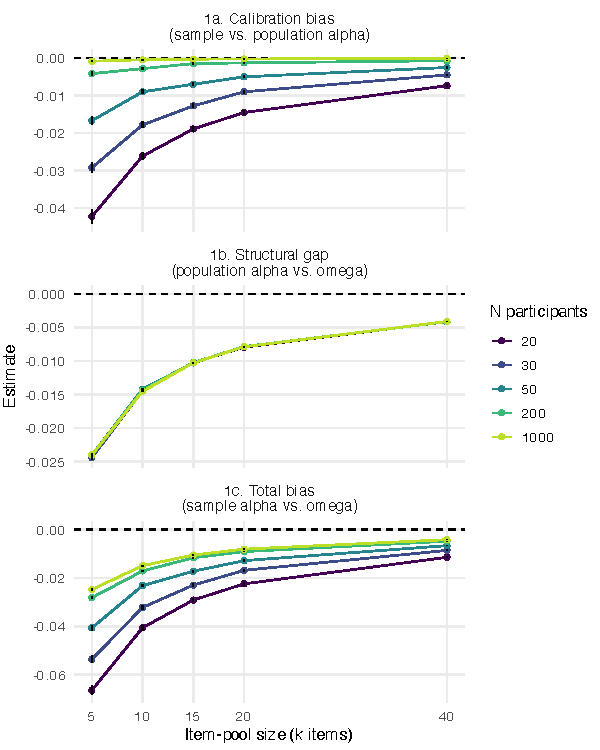
\includegraphics[width=1\linewidth,height=\textheight,keepaspectratio]{manuscript_files/figure-pdf/fig-fullpool-1.pdf}

}

\caption{\label{fig-fullpool}Full-pool calibration bias (1a), structural
gap between population alpha and omega (1b), and their sum, the total
bias against true reliability with no item dropping (1c), by item-pool
size (x axis) and sample size (colour). Error bars are +/-1 Monte Carlo
standard error and are narrower than the plotting symbol in most cells.
Note the differing y-axis scales. The structural gap (1b) depends only
on the loadings, so its five sample-size series coincide.}

\end{figure}%

\subsection{Bias in the reported alpha after item
dropping}\label{bias-in-the-reported-alpha-after-item-dropping}

\begingroup\fontsize{8}{10}\selectfont

\begin{longtable}[t]{lrrrrr}

\caption{\label{tbl-bias}Bias (+/-1 Monte Carlo standard error) of the
reported (sample) alpha of the retained items against the true
population alpha of those same items (2a) and against their true
reliability (2b), by strategy, item-pool size (k), and sample size (N).
The forced strategy drops in every replication by definition.
Conditional-strategy columns are marginal, so replications in which
nothing was dropped contribute the full-pool values.}

\tabularnewline

\toprule
\multicolumn{2}{c}{ } & \multicolumn{2}{c}{Forced} & \multicolumn{2}{c}{Conditional (marginal)} \\
\cmidrule(l{3pt}r{3pt}){3-4} \cmidrule(l{3pt}r{3pt}){5-6}
k & N & 2a vs. pop. alpha & 2b vs. reliability & 2a vs. pop. alpha & 2b vs. reliability\\
\midrule
\endfirsthead
\multicolumn{6}{@{}l}{\textit{(continued)}}\\
\toprule
\multicolumn{2}{c}{ } & \multicolumn{2}{c}{Forced} & \multicolumn{2}{c}{Conditional (marginal)} \\
\cmidrule(l{3pt}r{3pt}){3-4} \cmidrule(l{3pt}r{3pt}){5-6}
k & N & 2a vs. pop. alpha & 2b vs. reliability & 2a vs. pop. alpha & 2b vs. reliability\\
\midrule
\endhead

\endfoot
\bottomrule
\endlastfoot
 & 20 & 0.0435 (0.0013) & 0.0239 (0.0013) & 0.0415 (0.0013) & 0.0220 (0.0012)\\
\nopagebreak
 & 30 & 0.0315 (0.0011) & 0.0131 (0.0010) & 0.0293 (0.0010) & 0.0110 (0.0010)\\
\nopagebreak
 & 50 & 0.0228 (0.0008) & 0.0059 (0.0008) & 0.0211 (0.0008) & 0.0042 (0.0008)\\
\nopagebreak
 & 200 & 0.0064 (0.0004) & -0.0084 (0.0004) & 0.0057 (0.0004) & -0.0091 (0.0004)\\
\nopagebreak
\multirow[t]{-4}{*}[\normalbaselineskip]{\raggedright\arraybackslash 5} & 1000 & 0.0015 (0.0002) & -0.0123 (0.0002) & 0.0012 (0.0002) & -0.0125 (0.0002)\\
\cmidrule{1-6}\pagebreak[0]
 & 20 & 0.0057 (0.0008) & -0.0062 (0.0008) & 0.0056 (0.0008) & -0.0063 (0.0008)\\
\nopagebreak
 & 30 & 0.0045 (0.0006) & -0.0069 (0.0006) & 0.0044 (0.0006) & -0.0069 (0.0006)\\
\nopagebreak
 & 50 & 0.0048 (0.0005) & -0.0058 (0.0005) & 0.0048 (0.0005) & -0.0059 (0.0005)\\
\nopagebreak
 & 200 & 0.0009 (0.0002) & -0.0090 (0.0002) & 0.0008 (0.0002) & -0.0090 (0.0002)\\
\nopagebreak
\multirow[t]{-4}{*}[\normalbaselineskip]{\raggedright\arraybackslash 10} & 1000 & 0.0003 (0.0001) & -0.0093 (0.0001) & 0.0003 (0.0001) & -0.0093 (0.0001)\\
\cmidrule{1-6}\pagebreak[0]
 & 20 & -0.0017 (0.0006) & -0.0103 (0.0006) & -0.0017 (0.0006) & -0.0103 (0.0006)\\
\nopagebreak
 & 30 & -0.0008 (0.0004) & -0.0092 (0.0004) & -0.0008 (0.0004) & -0.0092 (0.0004)\\
\nopagebreak
 & 50 & 0.0003 (0.0003) & -0.0078 (0.0003) & 0.0003 (0.0003) & -0.0078 (0.0003)\\
\nopagebreak
 & 200 & 0.0005 (0.0002) & -0.0071 (0.0002) & 0.0005 (0.0002) & -0.0071 (0.0002)\\
\nopagebreak
\multirow[t]{-4}{*}[\normalbaselineskip]{\raggedright\arraybackslash 15} & 1000 & 0.0001 (0.0001) & -0.0073 (0.0001) & 0.0001 (0.0001) & -0.0073 (0.0001)\\
\cmidrule{1-6}\pagebreak[0]
 & 20 & -0.0035 (0.0005) & -0.0103 (0.0005) & -0.0035 (0.0005) & -0.0103 (0.0005)\\
\nopagebreak
 & 30 & -0.0015 (0.0003) & -0.0081 (0.0003) & -0.0015 (0.0003) & -0.0081 (0.0003)\\
\nopagebreak
 & 50 & -0.0004 (0.0003) & -0.0068 (0.0003) & -0.0004 (0.0003) & -0.0068 (0.0003)\\
\nopagebreak
 & 200 & -0.0000 (0.0001) & -0.0061 (0.0001) & -0.0000 (0.0001) & -0.0061 (0.0001)\\
\nopagebreak
\multirow[t]{-4}{*}[\normalbaselineskip]{\raggedright\arraybackslash 20} & 1000 & 0.0000 (0.0001) & -0.0059 (0.0001) & 0.0000 (0.0001) & -0.0059 (0.0001)\\
\cmidrule{1-6}\pagebreak[0]
 & 20 & -0.0039 (0.0002) & -0.0076 (0.0002) & -0.0039 (0.0002) & -0.0076 (0.0002)\\
\nopagebreak
 & 30 & -0.0021 (0.0002) & -0.0058 (0.0002) & -0.0021 (0.0002) & -0.0058 (0.0002)\\
\nopagebreak
 & 50 & -0.0010 (0.0001) & -0.0046 (0.0001) & -0.0010 (0.0001) & -0.0046 (0.0001)\\
\nopagebreak
 & 200 & -0.0003 (0.0001) & -0.0038 (0.0001) & -0.0003 (0.0001) & -0.0038 (0.0001)\\
\nopagebreak
\multirow[t]{-4}{*}[\normalbaselineskip]{\raggedright\arraybackslash 40} & 1000 & 0.0000 (0.0000) & -0.0034 (0.0000) & 0.0000 (0.0000) & -0.0034 (0.0000)\\*

\end{longtable}

\endgroup{}

Against the population \(\alpha\) of the retained items
(Table~\ref{tbl-bias}, column 2a), the selection-induced optimism
predicted by Kopalle \& Lehmann
(\citeproc{ref-kopalle_alpha_1997}{1997}) is clearly present at the
shortest scales, where the reported \(\alpha\) overstates the population
\(\alpha\) of the very items it describes by 0.0435 at \(k = 5\),
\(N = 20\). It shrinks rapidly with both factors, and at \(k \geq 15\)
with small samples it turns slightly negative, because the small-sample
downward calibration bias of \(\alpha\) documented above is then larger
than the optimism the argmax can extract from a pool that is already
long enough for \(\alpha\) to be estimated fairly stably. Selection
optimism is therefore not uniformly larger in longer scales, contrary to
the intuition that more candidate items means more opportunity to
capitalise on noise; with \(k\) items there are more candidates, but
each contributes proportionally less to \(\alpha\), and the second
effect dominates.

Against true reliability (column 2b), which is the applied target
because \(\alpha\) is reported as a reliability estimate, the two
components combine. The reported \(\alpha\) overstates true reliability
only in the shortest scales at small samples, in 3 of the 25 conditions,
all at \(k = 5\): by 0.0239 at \(N = 20\), falling to 0.0059 at
\(N = 50\). In every other condition it understates true reliability, by
between 0.003 and 0.012. The sign of the bias in a reported \(\alpha\)
after item dropping is therefore not fixed: it depends on where a given
study sits relative to selection optimism on one side and small-sample
calibration bias plus the structural gap on the other.

\begin{figure}

\centering{

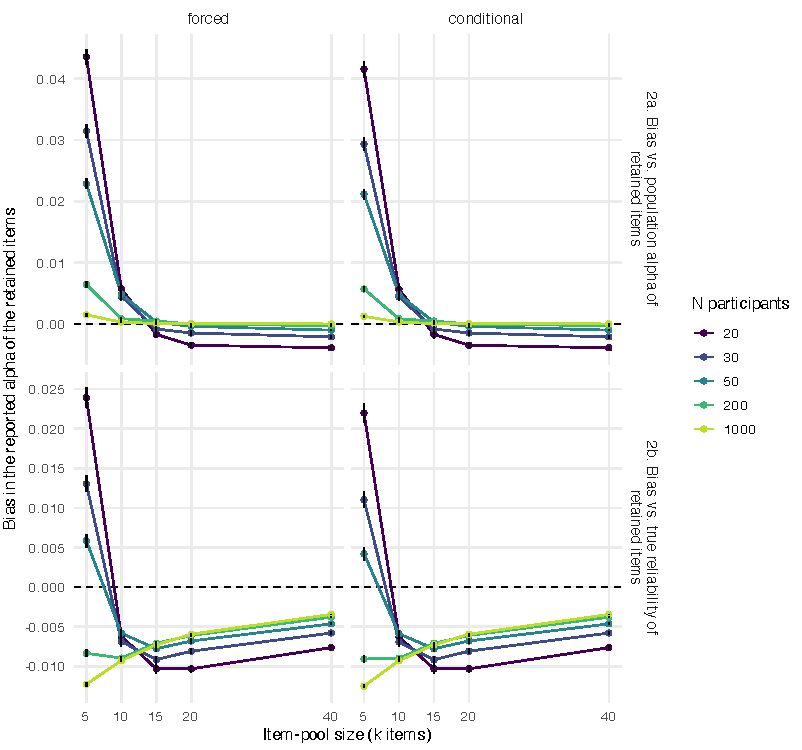
\includegraphics[width=1\linewidth,height=\textheight,keepaspectratio]{manuscript_files/figure-pdf/fig-bias-1.pdf}

}

\caption{\label{fig-bias}Bias in the reported alpha of the retained
items against the population alpha of those items (top row, 2a) and
against their true reliability (bottom row, 2b), for the forced (left)
and conditional (right) strategies, by item-pool size and sample size.
Error bars are +/-1 Monte Carlo standard error. The two strategies are
near-identical in every panel, consistent with their shared nomination
rule. Note the differing y-axis scales between rows.}

\end{figure}%

The same two estimands can be shown on the scale an applied reader
thinks in, which is also the form in which Kopalle \& Lehmann
(\citeproc{ref-kopalle_alpha_1997}{1997}) summarised their own results
and is therefore the directly comparable presentation: the true value of
the retained items on the horizontal axis, the reported sample
\(\alpha\) of those same items on the vertical axis, with the identity
line as the reference (Figure~\ref{fig-calibration}). Vertical distance
above the identity line is exactly the bias of estimand 2a (top row) or
2b (bottom row), and a no-dropping series is included so that the effect
of selection is visible against the baseline of not selecting at all.
Because every replication draws its own loadings, the true value varies
continuously within a condition rather than being fixed, so replications
are binned by it at a width of 0.05 and the mean reported \(\alpha\) is
plotted per bin; bins containing fewer than 20 replications are not
plotted, which removes 0.05\% of replications in the sparse tails of the
true-value distribution.

Two features are worth reading off it. First, the no-dropping series
does not lie on the identity line: against the population \(\alpha\) of
the retained items (top row) it sits below it, by 0.010 on average where
the true value exceeds 0.45 and by 0.025 where the true value is lower.
This is the small-sample calibration bias seen from a different angle,
and it is largest at low true values because those are the short, weakly
loaded pools whose covariances are estimated least precisely. Any
assessment of what selection does has to be read against that sloping
baseline rather than against the identity line.

Second, both dropping series sit above the no-dropping series
everywhere, and the vertical distance between them is the selection
effect in its purest form, since the three series differ only in whether
and how an item was chosen. At high true values that shift roughly
cancels the calibration bias, leaving the reported \(\alpha\) close to
correct (0.001 for the forced rule). At low true values it substantially
overshoots, leaving the reported \(\alpha\) 0.070 above the truth. This
is the Kopalle and Lehmann result in its original form, and it makes
clear that their ``alpha inflation'' is not a uniform upward shift but
something that bites hardest exactly where reliability is already poor.

The bottom row is the same replications compared against true
reliability instead. Every series moves down by the structural gap,
which is why the no-dropping series now sits 0.072 below the identity
line at low true values. Dropping partly offsets that displacement
rather than compounding it, which is the graphical form of the sign
reversal in Table~\ref{tbl-bias}: at high true values the forced rule
lands 0.007 below the truth, and only at low true values does it end up
above it (0.041).

These curves must not be read backwards. They give the expected reported
\(\alpha\) given the truth. The question an applied researcher faces is
the reverse one, since they know their reported \(\alpha\) and want the
truth, but the expected true value given a reported \(\alpha\) is a
different quantity that these curves do not provide, as it depends also
on how often each true value arises in the first place. Reading
horizontally from a reported \(\alpha\) across to a curve would
overstate what can be inferred from it.

\begin{figure}

\centering{

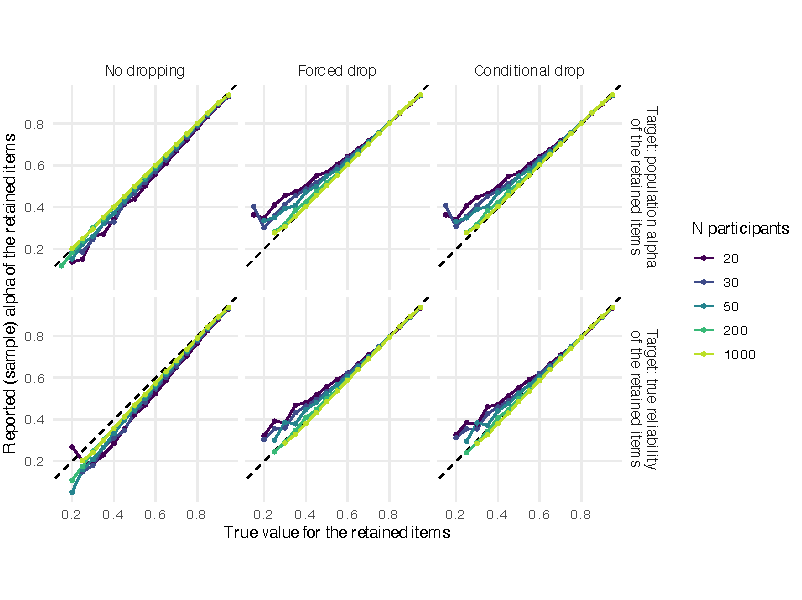
\includegraphics[width=1\linewidth,height=\textheight,keepaspectratio]{manuscript_files/figure-pdf/fig-calibration-1.pdf}

}

\caption{\label{fig-calibration}Calibration view: the reported (sample)
alpha of the retained items against their true value, in the
presentation used by Kopalle and Lehmann (1997). Columns are the two
dropping strategies plus a no-dropping reference; rows are the two
population targets. The dashed line is the identity: points on it mean
the reported alpha is exactly right for the items retained, and points
above it mean it overstates them. Replications are binned by their true
value at a width of 0.05 and averaged within bin; bins with fewer than
20 replications are omitted. Binning is presentational only and no
estimand is defined in terms of it.}

\end{figure}%

Restricting the conditional strategy to the replications in which it
actually acted (Table~\ref{tbl-givendrop}) leaves this pattern almost
unchanged, because both strategies remove the same nominated item
whenever the conditional strategy drops at all. The realised
\(K_{\text{drop}}\) shrinks furthest at the smallest pool size, where
the conditional rule declines to act increasingly often as \(N\) grows,
from 9.0\% of replications at \(N = 20\) to 22.1\% at \(N = 1000\). This
is consistent with greater sampling precision at larger \(N\) leaving
less noise for the argmax to exploit.

\begingroup\fontsize{8}{10}\selectfont

\begin{longtable}[t]{lrrrrr}

\caption{\label{tbl-givendrop}Conditional strategy, restricted to the
replications in which a drop actually occurred. Estimate (+/-1 Monte
Carlo standard error) of the bias in the reported alpha against
population alpha (2a) and against true reliability (2b), and the mean
true reliability change (3c). K(drop) is the realised number of
replications in which a drop occurred, out of 10,000.}

\tabularnewline

\toprule
k & N & K(drop) & 2a vs. pop. alpha & 2b vs. reliability & 3c. Reliability change\\
\midrule
\endfirsthead
\multicolumn{6}{@{}l}{\textit{(continued)}}\\
\toprule
k & N & K(drop) & 2a vs. pop. alpha & 2b vs. reliability & 3c. Reliability change\\
\midrule
\endhead

\endfoot
\bottomrule
\endlastfoot
 & 20 & 9,102 & 0.0391 (0.0014) & 0.0190 (0.0013) & 0.0023 (0.0005)\\
\nopagebreak
 & 30 & 8,868 & 0.0282 (0.0011) & 0.0091 (0.0011) & 0.0102 (0.0005)\\
\nopagebreak
 & 50 & 8,560 & 0.0209 (0.0009) & 0.0030 (0.0009) & 0.0167 (0.0004)\\
\nopagebreak
 & 200 & 8,013 & 0.0054 (0.0005) & -0.0109 (0.0005) & 0.0296 (0.0004)\\
\nopagebreak
\multirow[t]{-4}{*}[\normalbaselineskip]{\raggedright\arraybackslash 5} & 1000 & 7,794 & 0.0013 (0.0002) & -0.0143 (0.0003) & 0.0339 (0.0003)\\
\cmidrule{1-6}\pagebreak[0]
 & 20 & 9,874 & 0.0052 (0.0008) & -0.0067 (0.0008) & 0.0067 (0.0002)\\
\nopagebreak
 & 30 & 9,838 & 0.0041 (0.0006) & -0.0074 (0.0006) & 0.0089 (0.0002)\\
\nopagebreak
 & 50 & 9,750 & 0.0045 (0.0005) & -0.0063 (0.0005) & 0.0110 (0.0001)\\
\nopagebreak
 & 200 & 9,641 & 0.0007 (0.0002) & -0.0093 (0.0002) & 0.0146 (0.0001)\\
\nopagebreak
\multirow[t]{-4}{*}[\normalbaselineskip]{\raggedright\arraybackslash 10} & 1000 & 9,614 & 0.0003 (0.0001) & -0.0095 (0.0001) & 0.0159 (0.0001)\\
\cmidrule{1-6}\pagebreak[0]
 & 20 & 9,982 & -0.0017 (0.0006) & -0.0104 (0.0006) & 0.0051 (0.0001)\\
\nopagebreak
 & 30 & 9,978 & -0.0009 (0.0004) & -0.0092 (0.0004) & 0.0062 (0.0001)\\
\nopagebreak
 & 50 & 9,970 & 0.0003 (0.0003) & -0.0078 (0.0003) & 0.0073 (0.0001)\\
\nopagebreak
 & 200 & 9,939 & 0.0005 (0.0002) & -0.0071 (0.0002) & 0.0088 (0.0001)\\
\nopagebreak
\multirow[t]{-4}{*}[\normalbaselineskip]{\raggedright\arraybackslash 15} & 1000 & 9,919 & 0.0000 (0.0001) & -0.0073 (0.0001) & 0.0096 (0.0001)\\
\cmidrule{1-6}\pagebreak[0]
 & 20 & 9,999 & -0.0035 (0.0005) & -0.0103 (0.0005) & 0.0036 (0.0000)\\
\nopagebreak
 & 30 & 9,998 & -0.0015 (0.0003) & -0.0081 (0.0003) & 0.0043 (0.0000)\\
\nopagebreak
 & 50 & 9,993 & -0.0004 (0.0003) & -0.0068 (0.0003) & 0.0050 (0.0000)\\
\nopagebreak
 & 200 & 9,989 & -0.0000 (0.0001) & -0.0061 (0.0001) & 0.0059 (0.0000)\\
\nopagebreak
\multirow[t]{-4}{*}[\normalbaselineskip]{\raggedright\arraybackslash 20} & 1000 & 9,985 & 0.0000 (0.0001) & -0.0060 (0.0001) & 0.0063 (0.0000)\\
\cmidrule{1-6}\pagebreak[0]
 & 20 & 10,000 & -0.0039 (0.0002) & -0.0076 (0.0002) & 0.0014 (0.0000)\\
\nopagebreak
 & 30 & 10,000 & -0.0021 (0.0002) & -0.0058 (0.0002) & 0.0016 (0.0000)\\
\nopagebreak
 & 50 & 10,000 & -0.0010 (0.0001) & -0.0046 (0.0001) & 0.0018 (0.0000)\\
\nopagebreak
 & 200 & 10,000 & -0.0003 (0.0001) & -0.0038 (0.0001) & 0.0021 (0.0000)\\
\nopagebreak
\multirow[t]{-4}{*}[\normalbaselineskip]{\raggedright\arraybackslash 40} & 1000 & 10,000 & 0.0000 (0.0000) & -0.0034 (0.0000) & 0.0022 (0.0000)\\*

\end{longtable}

\endgroup{}

\subsection{Impact of item dropping}\label{impact-of-item-dropping}

Whether an item is dropped at all, and whether doing so helps or harms
the scale, are both determined by the number of items and the sample
size (Table~\ref{tbl-proportions}, Figure~\ref{fig-proportions}). The
propensity of the conditional strategy to drop an item is highest
exactly where its judgment is least trustworthy. At the smallest pool
size, \(\Pr(\text{drop})\) falls from 91.0\% at \(N = 20\) to 77.9\% at
\(N = 1000\). At the largest pool size it remains at or near 100\%
regardless of sample size: with more items available there is almost
always some single item whose removal raises the sample \(\alpha\),
whether or not that increase reflects a real improvement to the scale.

\begingroup\fontsize{8}{10}\selectfont

\begin{longtable}[t]{lrrrrr}

\caption{\label{tbl-proportions}Proportion of replications in which the
conditional strategy dropped an item (3e; the forced strategy drops in
all replications by definition), and the proportion in which the drop
reduced true reliability (3f, the harm rate), by strategy. All values
are percentages with +/-1 Monte Carlo standard error in percentage
points. The final column is the proportion of forced-strategy
replications in which the apparent in-sample gain was not positive,
i.e.~in which the drop did not even appear to help.}

\tabularnewline

\toprule
k & N & P(drop) & Harm, forced & Harm, cond. & No apparent gain, forced\\
\midrule
\endfirsthead
\multicolumn{6}{@{}l}{\textit{(continued)}}\\
\toprule
k & N & P(drop) & Harm, forced & Harm, cond. & No apparent gain, forced\\
\midrule
\endhead

\endfoot
\bottomrule
\endlastfoot
 & 20 & 91.0 (0.29) & 49.6 (0.50) & 42.5 (0.49) & 9.0\\
\nopagebreak
 & 30 & 88.7 (0.32) & 43.9 (0.50) & 34.9 (0.48) & 11.3\\
\nopagebreak
 & 50 & 85.6 (0.35) & 39.3 (0.49) & 28.3 (0.45) & 14.4\\
\nopagebreak
 & 200 & 80.1 (0.40) & 28.9 (0.45) & 12.8 (0.33) & 19.9\\
\nopagebreak
\multirow[t]{-4}{*}[\normalbaselineskip]{\raggedright\arraybackslash 5} & 1000 & 77.9 (0.41) & 25.3 (0.43) & 5.6 (0.23) & 22.1\\
\cmidrule{1-6}\pagebreak[0]
 & 20 & 98.7 (0.11) & 32.7 (0.47) & 31.6 (0.47) & 1.3\\
\nopagebreak
 & 30 & 98.4 (0.13) & 27.6 (0.45) & 26.5 (0.44) & 1.6\\
\nopagebreak
 & 50 & 97.5 (0.16) & 21.1 (0.41) & 19.4 (0.40) & 2.5\\
\nopagebreak
 & 200 & 96.4 (0.19) & 10.0 (0.30) & 7.4 (0.26) & 3.6\\
\nopagebreak
\multirow[t]{-4}{*}[\normalbaselineskip]{\raggedright\arraybackslash 10} & 1000 & 96.1 (0.19) & 5.6 (0.23) & 2.4 (0.15) & 3.9\\
\cmidrule{1-6}\pagebreak[0]
 & 20 & 99.8 (0.04) & 25.1 (0.43) & 24.9 (0.43) & 0.2\\
\nopagebreak
 & 30 & 99.8 (0.05) & 19.1 (0.39) & 19.0 (0.39) & 0.2\\
\nopagebreak
 & 50 & 99.7 (0.05) & 13.0 (0.34) & 12.8 (0.33) & 0.3\\
\nopagebreak
 & 200 & 99.4 (0.08) & 4.1 (0.20) & 3.6 (0.19) & 0.6\\
\nopagebreak
\multirow[t]{-4}{*}[\normalbaselineskip]{\raggedright\arraybackslash 15} & 1000 & 99.2 (0.09) & 1.4 (0.12) & 0.8 (0.09) & 0.8\\
\cmidrule{1-6}\pagebreak[0]
 & 20 & 100.0 (0.01) & 20.4 (0.40) & 20.4 (0.40) & 0.0\\
\nopagebreak
 & 30 & 100.0 (0.01) & 15.2 (0.36) & 15.2 (0.36) & 0.0\\
\nopagebreak
 & 50 & 99.9 (0.03) & 8.9 (0.28) & 8.9 (0.28) & 0.1\\
\nopagebreak
 & 200 & 99.9 (0.03) & 1.9 (0.14) & 1.8 (0.13) & 0.1\\
\nopagebreak
\multirow[t]{-4}{*}[\normalbaselineskip]{\raggedright\arraybackslash 20} & 1000 & 99.9 (0.04) & 0.4 (0.07) & 0.3 (0.06) & 0.1\\
\cmidrule{1-6}\pagebreak[0]
 & 20 & 100.0 (0.00) & 12.0 (0.33) & 12.0 (0.33) & 0.0\\
\nopagebreak
 & 30 & 100.0 (0.00) & 7.0 (0.26) & 7.0 (0.26) & 0.0\\
\nopagebreak
 & 50 & 100.0 (0.00) & 3.2 (0.18) & 3.2 (0.18) & 0.0\\
\nopagebreak
 & 200 & 100.0 (0.00) & 0.1 (0.04) & 0.1 (0.04) & 0.0\\
\nopagebreak
\multirow[t]{-4}{*}[\normalbaselineskip]{\raggedright\arraybackslash 40} & 1000 & 100.0 (0.00) & 0.0 (0.00) & 0.0 (0.00) & 0.0\\*

\end{longtable}

\endgroup{}

The consequences of removing the item are given by the harm rate, the
proportion of replications in which the drop reduced true reliability.
At the smallest scale and sample size the forced strategy's harm rate is
49.6\%: the nominated item is very nearly as likely to be an artefact of
that particular sample as it is to be a genuine weak point in the scale.
Harm falls steeply as either factor increases, but it does not vanish
with sample size alone. At \(N = 1000\) the forced strategy still
reduces true reliability in 25.3\% of replications at \(k = 5\), and the
rate reaches 0.0\% only in the largest scale and sample combination.
Long scales and large samples are both needed; neither alone is
sufficient.

The harm rate for the conditional strategy is lower than for the forced
strategy in every condition (42.5\% versus 49.6\% at \(k = 5\),
\(N = 20\)), because declining to act in the replications with the
weakest apparent improvement disproportionately screens out cases that
would otherwise have reduced reliability. This lowers the incidence of
harm across all studies, not the risk in the studies where the item is
dropped. The gating rule is a filter on how often the gamble is taken,
not on whether it pays off.

An important qualification concerns how the harm rate should be
described. It is tempting to say the drop harms reliability ``while
appearing to improve \(\alpha\) every time'', but this holds only for
the conditional strategy, for which
\(\widehat{\Delta}_{\text{obs}} > 0\) is true by construction whenever
it acts. The forced strategy has no such guarantee: its apparent gain
was not positive in 9.0\% of replications at \(k = 5\), \(N = 20\),
rising to 22.1\% at \(N = 1000\) (Table~\ref{tbl-proportions}, final
column). The strongest claim the design supports without qualification
is therefore the conditional one: at \(k = 5\), \(N = 20\), the rule
that acts only when the in-sample \(\alpha\) improves nevertheless
reduced true reliability in 42.5\% of the replications in which it
acted.

\begin{figure}

\centering{

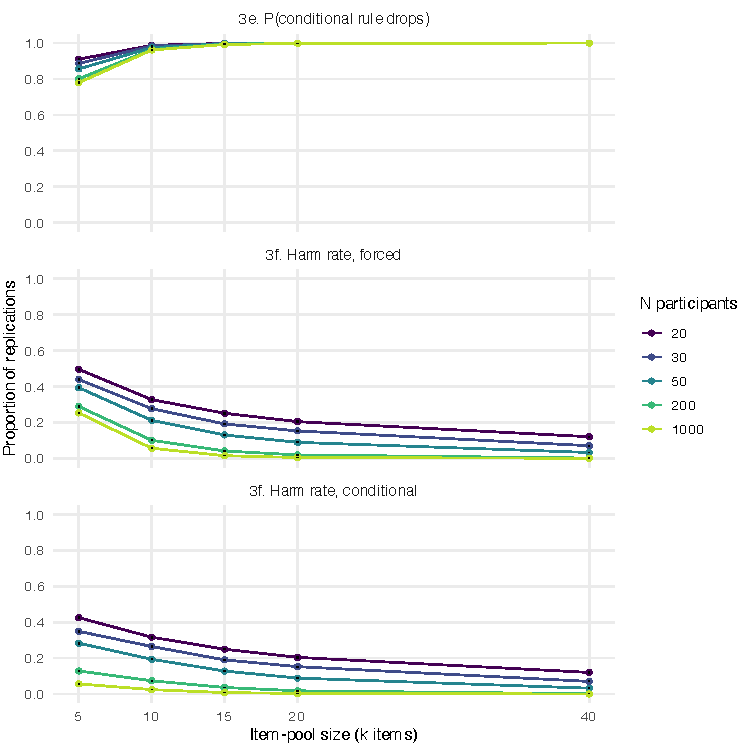
\includegraphics[width=1\linewidth,height=\textheight,keepaspectratio]{manuscript_files/figure-pdf/fig-proportions-1.pdf}

}

\caption{\label{fig-proportions}Probability that the conditional
strategy drops an item (left) and the probability that the drop reduced
true reliability, i.e.~the harm rate, for each strategy (centre and
right), by item-pool size and sample size. Error bars are +/-1 Monte
Carlo standard error. The conditions in which the conditional rule is
most likely to act are the conditions in which acting is most likely to
harm the scale.}

\end{figure}%

The same pattern appears in the magnitude of what item dropping does to
the scale (Table~\ref{tbl-deltas}). The observed sample gain
\(\widehat{\Delta}_{\text{obs}}\) is positive on average in every
condition, including those with the highest harm rates. The population
\(\alpha\) change \(\Delta_{\text{pop}}\) and the true reliability
change \(\Delta_{\rho}\) are both consistently smaller, and the gap
between \(\widehat{\Delta}_{\text{obs}}\) and \(\Delta_{\text{pop}}\),
the selection optimism, is largest exactly where the harm rate is
highest: 0.086 at \(k = 5\), \(N = 20\), falling to 0.0001 at
\(k = 40\), \(N = 1000\). The conditions producing the most inflated
apparent gain are the same conditions producing the highest probability
that the underlying decision was actively counterproductive. Most
strikingly, at \(k = 5\), \(N = 20\) the forced rule's mean apparent
gain of 0.090 in sample \(\alpha\) corresponds to a mean change in true
reliability of -0.0007, which is to say essentially none at all: almost
the entire apparent improvement is selection optimism.

\begingroup\fontsize{8}{10}\selectfont

\begin{longtable}[t]{lrrrrr}

\caption{\label{tbl-deltas}Mean change (+/-1 Monte Carlo standard error)
from full pool to retained items on three scales -- observed sample
alpha (3a), population alpha (3b), and true reliability (3c) -- together
with the selection optimism (3d = 3a - 3b, computed pairwise within
replicate), for the forced strategy, by item-pool size (k) and sample
size (N). Conditional-strategy values are given in the compendium; they
differ only through the replications in which no drop occurred, which
contribute zeros.}

\tabularnewline

\toprule
k & N & 3a. Observed & 3b. Population alpha & 3c. True reliability & 3d. Optimism\\
\midrule
\endfirsthead
\multicolumn{6}{@{}l}{\textit{(continued)}}\\
\toprule
k & N & 3a. Observed & 3b. Population alpha & 3c. True reliability & 3d. Optimism\\
\midrule
\endhead

\endfoot
\bottomrule
\endlastfoot
 & 20 & 0.0897 (0.0011) & 0.0038 (0.0006) & -0.0007 (0.0005) & 0.0858 (0.0010)\\
\nopagebreak
 & 30 & 0.0726 (0.0008) & 0.0118 (0.0006) & 0.0058 (0.0005) & 0.0607 (0.0008)\\
\nopagebreak
 & 50 & 0.0576 (0.0007) & 0.0180 (0.0006) & 0.0110 (0.0004) & 0.0395 (0.0006)\\
\nopagebreak
 & 200 & 0.0404 (0.0005) & 0.0298 (0.0005) & 0.0206 (0.0003) & 0.0106 (0.0003)\\
\nopagebreak
\multirow[t]{-4}{*}[\normalbaselineskip]{\raggedright\arraybackslash 5} & 1000 & 0.0359 (0.0005) & 0.0336 (0.0005) & 0.0234 (0.0003) & 0.0023 (0.0001)\\
\cmidrule{1-6}\pagebreak[0]
 & 20 & 0.0409 (0.0004) & 0.0090 (0.0002) & 0.0065 (0.0002) & 0.0319 (0.0004)\\
\nopagebreak
 & 30 & 0.0340 (0.0003) & 0.0116 (0.0002) & 0.0086 (0.0002) & 0.0223 (0.0003)\\
\nopagebreak
 & 50 & 0.0279 (0.0002) & 0.0141 (0.0002) & 0.0106 (0.0001) & 0.0138 (0.0002)\\
\nopagebreak
 & 200 & 0.0221 (0.0002) & 0.0184 (0.0002) & 0.0139 (0.0001) & 0.0037 (0.0001)\\
\nopagebreak
\multirow[t]{-4}{*}[\normalbaselineskip]{\raggedright\arraybackslash 10} & 1000 & 0.0209 (0.0002) & 0.0201 (0.0002) & 0.0152 (0.0001) & 0.0007 (0.0000)\\
\cmidrule{1-6}\pagebreak[0]
 & 20 & 0.0239 (0.0002) & 0.0067 (0.0001) & 0.0051 (0.0001) & 0.0172 (0.0002)\\
\nopagebreak
 & 30 & 0.0200 (0.0001) & 0.0080 (0.0001) & 0.0061 (0.0001) & 0.0119 (0.0001)\\
\nopagebreak
 & 50 & 0.0167 (0.0001) & 0.0095 (0.0001) & 0.0072 (0.0001) & 0.0073 (0.0001)\\
\nopagebreak
 & 200 & 0.0134 (0.0001) & 0.0115 (0.0001) & 0.0088 (0.0001) & 0.0019 (0.0000)\\
\nopagebreak
\multirow[t]{-4}{*}[\normalbaselineskip]{\raggedright\arraybackslash 15} & 1000 & 0.0127 (0.0001) & 0.0124 (0.0001) & 0.0095 (0.0001) & 0.0003 (0.0000)\\
\cmidrule{1-6}\pagebreak[0]
 & 20 & 0.0158 (0.0001) & 0.0047 (0.0001) & 0.0036 (0.0000) & 0.0111 (0.0001)\\
\nopagebreak
 & 30 & 0.0131 (0.0001) & 0.0056 (0.0001) & 0.0043 (0.0000) & 0.0075 (0.0001)\\
\nopagebreak
 & 50 & 0.0110 (0.0001) & 0.0064 (0.0001) & 0.0050 (0.0000) & 0.0046 (0.0001)\\
\nopagebreak
 & 200 & 0.0090 (0.0001) & 0.0077 (0.0000) & 0.0059 (0.0000) & 0.0012 (0.0000)\\
\nopagebreak
\multirow[t]{-4}{*}[\normalbaselineskip]{\raggedright\arraybackslash 20} & 1000 & 0.0085 (0.0000) & 0.0082 (0.0000) & 0.0063 (0.0000) & 0.0002 (0.0000)\\
\cmidrule{1-6}\pagebreak[0]
 & 20 & 0.0052 (0.0000) & 0.0017 (0.0000) & 0.0014 (0.0000) & 0.0035 (0.0000)\\
\nopagebreak
 & 30 & 0.0044 (0.0000) & 0.0020 (0.0000) & 0.0016 (0.0000) & 0.0024 (0.0000)\\
\nopagebreak
 & 50 & 0.0038 (0.0000) & 0.0023 (0.0000) & 0.0018 (0.0000) & 0.0015 (0.0000)\\
\nopagebreak
 & 200 & 0.0031 (0.0000) & 0.0027 (0.0000) & 0.0021 (0.0000) & 0.0004 (0.0000)\\
\nopagebreak
\multirow[t]{-4}{*}[\normalbaselineskip]{\raggedright\arraybackslash 40} & 1000 & 0.0029 (0.0000) & 0.0029 (0.0000) & 0.0022 (0.0000) & 0.0001 (0.0000)\\*

\end{longtable}

\endgroup{}

\subsection{What a single study can
encounter}\label{what-a-single-study-can-encounter}

Every quantity above is a long-run average over 10,000 replications. The
prediction intervals in Table~\ref{tbl-pi} and Figure~\ref{fig-pi}
describe the spread instead: the range of outcomes a single study, run
once under this rule, can encounter.

\clearpage
\begin{landscape}

\begingroup\fontsize{8}{10}\selectfont

\begin{longtable}[t]{lrrrr}

\caption{\label{tbl-pi}Mean {[}95\% prediction interval{]} of each
per-replication quantity, for the forced strategy, by item-pool size (k)
and sample size (N). The interval is the empirical 2.5th to 97.5th
percentile range across the 10,000 replications of a condition. It
describes the spread across individual studies, not the precision of the
mean, and unlike a Monte Carlo standard error it does not shrink as the
number of replications grows.}

\tabularnewline

\toprule
k & N & 3a. Observed gain & 3c. True reliability change & 2b. Bias vs. reliability\\
\midrule
\endfirsthead
\multicolumn{5}{@{}l}{\textit{(continued)}}\\
\toprule
k & N & 3a. Observed gain & 3c. True reliability change & 2b. Bias vs. reliability\\
\midrule
\endhead

\endfoot
\bottomrule
\endlastfoot
 & 20 & 0.090 [-0.013, 0.360] & -0.001 [-0.107, 0.094] & 0.024 [-0.267, 0.243]\\
\nopagebreak
 & 30 & 0.073 [-0.017, 0.289] & 0.006 [-0.090, 0.097] & 0.013 [-0.221, 0.199]\\
\nopagebreak
 & 50 & 0.058 [-0.019, 0.227] & 0.011 [-0.074, 0.097] & 0.006 [-0.173, 0.159]\\
\nopagebreak
 & 200 & 0.040 [-0.024, 0.166] & 0.021 [-0.040, 0.099] & -0.008 [-0.103, 0.073]\\
\nopagebreak
\multirow[t]{-4}{*}[\normalbaselineskip]{\raggedright\arraybackslash 5} & 1000 & 0.036 [-0.025, 0.155] & 0.023 [-0.028, 0.099] & -0.012 [-0.065, 0.027]\\
\cmidrule{1-5}\pagebreak[0]
 & 20 & 0.041 [0.002, 0.138] & 0.006 [-0.025, 0.039] & -0.006 [-0.199, 0.111]\\
\nopagebreak
 & 30 & 0.034 [0.001, 0.110] & 0.009 [-0.019, 0.040] & -0.007 [-0.155, 0.093]\\
\nopagebreak
 & 50 & 0.028 [0.000, 0.085] & 0.011 [-0.015, 0.040] & -0.006 [-0.114, 0.073]\\
\nopagebreak
 & 200 & 0.022 [-0.001, 0.066] & 0.014 [-0.006, 0.041] & -0.009 [-0.063, 0.034]\\
\nopagebreak
\multirow[t]{-4}{*}[\normalbaselineskip]{\raggedright\arraybackslash 10} & 1000 & 0.021 [-0.001, 0.062] & 0.015 [-0.002, 0.043] & -0.009 [-0.036, 0.011]\\
\cmidrule{1-5}\pagebreak[0]
 & 20 & 0.024 [0.003, 0.075] & 0.005 [-0.010, 0.021] & -0.010 [-0.156, 0.072]\\
\nopagebreak
 & 30 & 0.020 [0.003, 0.057] & 0.006 [-0.007, 0.022] & -0.009 [-0.116, 0.061]\\
\nopagebreak
 & 50 & 0.017 [0.002, 0.046] & 0.007 [-0.005, 0.023] & -0.008 [-0.088, 0.047]\\
\nopagebreak
 & 200 & 0.013 [0.002, 0.035] & 0.009 [-0.001, 0.023] & -0.007 [-0.044, 0.022]\\
\nopagebreak
\multirow[t]{-4}{*}[\normalbaselineskip]{\raggedright\arraybackslash 15} & 1000 & 0.013 [0.001, 0.033] & 0.009 [0.001, 0.023] & -0.007 [-0.025, 0.007]\\
\cmidrule{1-5}\pagebreak[0]
 & 20 & 0.016 [0.003, 0.047] & 0.004 [-0.005, 0.013] & -0.010 [-0.122, 0.053]\\
\nopagebreak
 & 30 & 0.013 [0.003, 0.035] & 0.004 [-0.004, 0.014] & -0.008 [-0.093, 0.044]\\
\nopagebreak
 & 50 & 0.011 [0.002, 0.028] & 0.005 [-0.002, 0.014] & -0.007 [-0.066, 0.035]\\
\nopagebreak
 & 200 & 0.009 [0.002, 0.021] & 0.006 [0.000, 0.014] & -0.006 [-0.034, 0.016]\\
\nopagebreak
\multirow[t]{-4}{*}[\normalbaselineskip]{\raggedright\arraybackslash 20} & 1000 & 0.008 [0.002, 0.020] & 0.006 [0.001, 0.014] & -0.006 [-0.019, 0.005]\\
\cmidrule{1-5}\pagebreak[0]
 & 20 & 0.005 [0.001, 0.014] & 0.001 [-0.001, 0.004] & -0.008 [-0.070, 0.025]\\
\nopagebreak
 & 30 & 0.004 [0.001, 0.010] & 0.002 [-0.001, 0.004] & -0.006 [-0.051, 0.021]\\
\nopagebreak
 & 50 & 0.004 [0.001, 0.008] & 0.002 [-0.000, 0.004] & -0.005 [-0.036, 0.017]\\
\nopagebreak
 & 200 & 0.003 [0.001, 0.006] & 0.002 [0.001, 0.004] & -0.004 [-0.018, 0.008]\\
\nopagebreak
\multirow[t]{-4}{*}[\normalbaselineskip]{\raggedright\arraybackslash 40} & 1000 & 0.003 [0.001, 0.006] & 0.002 [0.001, 0.004] & -0.003 [-0.010, 0.002]\\*

\end{longtable}

\endgroup{}

\end{landscape}
\clearpage

The intervals narrow sharply as either design factor grows. For the bias
in the reported \(\alpha\) against true reliability, the interval spans
0.510 at \(k = 5\), \(N = 20\) ({[}-0.267, 0.243{]}) and only 0.012 at
\(k = 40\), \(N = 1000\) ({[}-0.010, 0.002{]}). The true reliability
change narrows correspondingly, from 0.200 to 0.003 wide.

The gap between these intervals and the corresponding Monte Carlo
standard errors is the substantive point of this aim. At \(k = 5\),
\(N = 20\), the mean bias against true reliability is 0.024 with a Monte
Carlo standard error of 0.0013, so the long-run average is pinned down
to within a thousandth. Yet the individual studies making up that
average span {[}-0.267, 0.243{]}, a range roughly 404 times wider than
the standard error.

That ratio is not a finding about item dropping; it is close to an
identity. For any approximately normal quantity the interval width is
about \(3.92 S_d\) while the standard error is \(S_d/\sqrt{K}\), so
their ratio is about \(3.92\sqrt{K} \approx 392\) at \(K\) = 10,000
regardless of the condition, and indeed it varies only between 345 and
424 across the entire design. That is exactly why it matters. Running
more replications raises this ratio rather than lowering it: the
precision of the reported mean and the spread that an individual study
faces are not merely different in size, they move in opposite directions
as a simulation is scaled up. A researcher reporting an \(\alpha\) after
dropping an item from a five-item scale measured on twenty participants
is drawing from the wide distribution, not from a neighbourhood of the
mean, and no amount of additional simulation narrows what they face.

\begin{figure}

\centering{

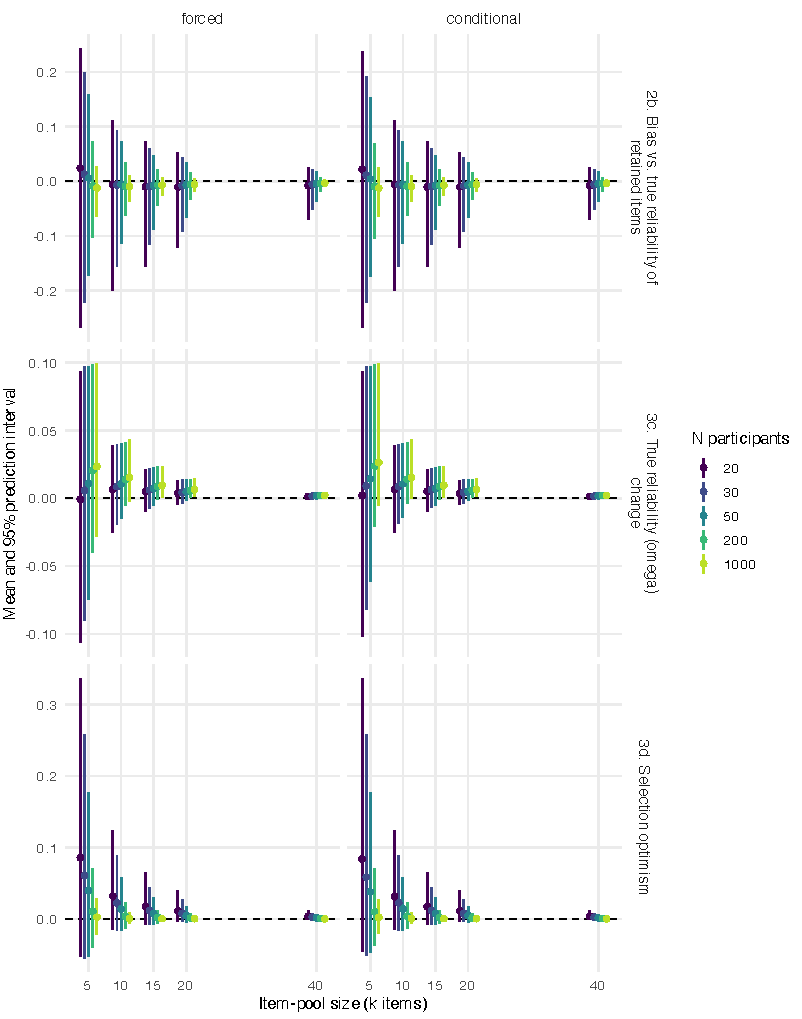
\includegraphics[width=1\linewidth,height=\textheight,keepaspectratio]{manuscript_files/figure-pdf/fig-pi-1.pdf}

}

\caption{\label{fig-pi}Mean and 95\% prediction interval for the bias in
the reported alpha against true reliability (top), the true reliability
change (middle), and the selection optimism (bottom), for the forced
(left) and conditional (right) strategies, by item-pool size and sample
size. Points are means; bars span the empirical 2.5th to 97.5th
percentiles across replications. Bars are dodged horizontally within
each item-pool size so the five sample sizes are distinguishable. Note
the differing y-axis scales between rows.}

\end{figure}%

\section{Discussion}\label{discussion}

Four things follow from these results. First, \(\alpha\) has two
independent reasons to be untrustworthy before any item is dropped at
all: ordinary small-sample noise, which fades with \(N\) (from -0.042 at
\(N = 20\) to -0.0008 at \(N = 1000\) for \(k = 5\)), and a structural
ceiling on what \(\alpha\) can measure relative to true reliability,
which does not fade with \(N\) at all, only with \(k\) (from -0.024 at
\(k = 5\) to -0.004 at \(k = 40\)). Second, introducing the selection
step adds a third source of distortion that interacts with the first two
and flips the overall sign of the bias depending on where in the design
a study sits. Third, the bias in the number is almost beside the point:
the decision itself is frequently wrong in the sense that matters,
degrading true reliability. Fourth, none of these averages is a safe
guide to what any one real study will observe.

\subsection{What we expected, and what we
found}\label{what-we-expected-and-what-we-found}

Because this simulation was not preregistered, the expectations recorded
in the Method are priors rather than tests, and we set them against the
results explicitly so that the reader can see which parts of the account
were anticipated and which were not.

Three expectations held straightforwardly. The full-pool calibration
bias was small, negative, and shrank toward zero with \(N\) at every
item-pool size. The structural gap was negative in every one of the 25
conditions. And the prediction intervals were wide relative to the means
wherever selection had room to operate, narrowing as either design
factor grew.

One expectation was clearly wrong, and its being wrong is informative.
We expected selection optimism to be larger at larger item-pool sizes,
reasoning that more candidate items gives a larger expected maximum over
noise. The opposite holds: the bias against the population \(\alpha\) of
the retained items is largest at \(k = 5\) (0.0435 at \(N = 20\)) and is
already slightly negative at \(k \geq 15\) with small samples. Our
reasoning counted the number of candidates and ignored their individual
leverage. With more items each contributes proportionally less to
\(\alpha\), so the maximum is taken over a larger set of individually
smaller perturbations, and the second effect dominates. It is also
swamped, at longer pools, by the small-sample downward calibration bias
pulling in the opposite direction. The practical implication runs
opposite to the intuition: long scales are not more exploitable by this
rule, they are less so.

A second expectation was right in direction but badly wrong in emphasis.
We expected the reliability-scale bias to be negative at large \(N\) and
possibly positive at small \(N\), and treated the location of the sign
change as the open question. It is positive in only 3 of 25 conditions,
all at the shortest pool size, so the sign change is real but confined
to a corner of the design. Framing the study around it, as an ``alpha
inflation'' account would, would have been a mistake. Across most of the
grid the reported number is only slightly wrong, and had we stopped at
the estimands we thought would carry the paper, we would have concluded
that item dropping is a minor problem. The harm rate, for which we
deliberately made no directional prediction because we could not
anticipate the balance between genuinely bad items and pure length
penalties, is what shows otherwise: up to 49.6\% of replications made
worse. The finding we did not predict is the one that matters, and it is
measured by an estimand we included precisely because we did not know
what it would show.

Finally, \(\Pr(\text{drop})\) rose with item-pool size as expected, but
its behaviour in \(N\) was the informative part and we had not thought
it through in advance. It falls as \(N\) grows at short pool sizes, from
91.0\% to 77.9\%, because noise-driven drops die out with sampling
precision and only genuinely harmful items are left to remove. The rule
therefore fires most often exactly where its firing means least.

\subsection{Reconciling with the simulation
literature}\label{reconciling-with-the-simulation-literature}

Kopalle \& Lehmann (\citeproc{ref-kopalle_alpha_1997}{1997}) established
that item selection based on the same sample subsequently used to report
the resulting \(\alpha\) capitalises on chance. The present work
reproduces that finding where the item pool and sample are both small,
and qualifies it elsewhere. Measured against the population \(\alpha\)
of the retained items, the optimism is unambiguous at \(k = 5\) but has
essentially vanished by \(k = 15\), where it is outweighed by the
opposing small-sample calibration bias. Measured against true
reliability, which is the quantity researchers care about, the sign
reverses across most of the design. The direction of bias in an
\(\alpha\) reported after item dropping is therefore not fixed, and an
unqualified ``alpha inflation'' framing does not survive contact with a
design that varies scale length and sample size over realistic ranges
and evaluates against reliability rather than against \(\alpha\) itself.

The finding that \(\alpha\) and true reliability diverge even with no
item selection at all is consistent with a separate, long-running
critique of Cronbach's \(\alpha\). Sijtsma
(\citeproc{ref-sijtsma_use_2009}{2009}) argued that \(\alpha\) cannot in
general equal the true reliability of a scale given its inter-item
covariance structure, a point developed in the \(\alpha\)/\(\omega\)
literature (\citeproc{ref-mcdonald_test_1999}{McDonald, 1999};
\citeproc{ref-revelle_coefficients_2009}{Revelle \& Zinbarg, 2009};
\citeproc{ref-zinbarg_cronbachs_2005}{Zinbarg et al., 2005}), which
shows the two coefficients are equal only under the restrictive
condition of essentially equal item loadings. Our structural-gap result
is a direct simulation demonstration of that theoretical point under an
empirically calibrated loading distribution, and shows its magnitude is
not negligible relative to the biases usually discussed in the
item-dropping literature. At the shortest scale examined it is 0.024,
which exceeds the selection optimism observed anywhere in the design
outside the \(k = 5\) column.

\subsection{Bias in the reported number versus harm to the
scale}\label{bias-in-the-reported-number-versus-harm-to-the-scale}

The most consequential finding is not that the reported number is wrong.
Across most of the design it is only slightly wrong, with magnitudes
mostly under 0.01. It is that the decision itself is frequently
detrimental. In the worst condition, the forced rule reduced true
reliability in 49.6\% of replications while its mean apparent in-sample
gain was 0.090; the conditional rule, which acts only on an apparent
improvement, still did so in 42.5\% of the replications in which it
acted.

A modest average bias can coexist with a near-coin-flip probability of a
harmful outcome, because the bias measure averages over both helpful and
harmful replications while the harm rate isolates how often the harmful
case occurs. Nothing about the reported \(\alpha\) itself distinguishes
the two scenarios.

This bears on how the downstream result should be read. Stefan \&
Schönbrodt (\citeproc{ref-stefan_big_2023}{2023}) show that item
dropping on \(\alpha\) inflates the false positive rate of the
subsequent hypothesis test to as high as 30\%, and it would be natural
to attribute that to the reported reliability being overstated. These
results suggest that is largely not the mechanism: across most of the
design the reported \(\alpha\) is close to correct, and in the majority
of conditions it is too low rather than too high. What the practice
supplies instead is a decision point at which the analyst may retain
either of two scales, taken after seeing the data, in conditions where
the two are close to indistinguishable on the evidence available. The
inflation is better understood as an experimenter degree of freedom than
as a mis-estimated reliability, which matters because the two call for
different remedies: reporting \(\omega\) instead of \(\alpha\) would
address the second and not the first. This is also why the average is
the wrong summary to lead with for practice: a mean \(\Delta_\rho\) of
-0.0007 at \(k = 5\), \(N = 20\) reads as ``no effect'' but is the
average of a distribution in which roughly half of studies are made
worse and roughly half are made better.

\subsection{Mean bias understates practical
risk}\label{mean-bias-understates-practical-risk}

A mean bias near zero is compatible either with every study landing
close to zero or with studies scattered across a wide range that happens
to average out there. Table~\ref{tbl-pi} shows the design is
unambiguously the second case for short scales: the \(k = 5\),
\(N = 20\) cell alone spans {[}-0.267, 0.243{]}. Additional Monte Carlo
replications would narrow the standard error on the mean further but
would not narrow this interval by anything, since it is a property of
the distribution rather than of how many times we sampled from it.
Reporting means with Monte Carlo standard errors alone, which is common
practice in simulation studies, would understate what item dropping can
do in a single study by a factor of roughly 392 here, and by a larger
factor still in any simulation run with more replications.

\subsection{Practical implications}\label{practical-implications}

In short scales and small samples, precisely where the reported number
is most likely to be optimistically biased, the underlying decision is
most likely to be actively wrong. Previous simulation findings have
shown that unbiased estimation of \(\alpha\) at small \(N\) is possible
when the largest eigenvalue of the item covariance matrix is large
(\citeproc{ref-yurdugul_minimum_2008}{Yurdugül, 2008}), indicating that
bias in \(\alpha\) depends on how strongly unidimensional the items are
as well as on sample size. As short scales are by construction more
likely to be unidimensional, this qualifies but does not remove the
practical concern raised here.

The key distinction for measurement practice is between what is knowable
before a study is run and what is knowable after. Scale length and
sample size are properties of the study design. Everything this
simulation quantifies as risky, that is, the optimistic bias, the harm
rate, and the width of the prediction interval, is a function of those
two design choices and of nothing about the data subsequently collected.
The risk can therefore be known in advance: a researcher could take a
proposed \(k\) and \(N\), find the corresponding row of
Table~\ref{tbl-proportions}, and know before collecting data roughly how
much to trust a future item-dropping decision from that study. This is
an unusual property for a bias to have. Many statistical biases depend
on unknown population parameters that the researcher cannot inspect in
advance; this one depends only on design choices that are already
written down in the preregistration or method section.

What cannot be known in advance is anything from inside the
alpha-if-item-removed table itself. The table that
\texttt{psych::alpha()}, or any equivalent, produces looks exactly the
same whether the item it nominates is genuinely the weakest link in the
scale or is the item that happened to draw an unfavourable sample of
participants this time. It carries no confidence interval and no
indication of ranking instability. Two researchers who drew two
different samples of the same size from the same true scale would each
see a complete, definitive-looking table, possibly nominating different
items for removal, and each would have exactly the same apparent
justification for acting on it, even though at most one of them has
observed real signal. The safeguard has to come from knowing where \(k\)
and \(N\) sit in a risk table such as Table~\ref{tbl-proportions},
because nothing internal to the analysis will indicate the risk level.

\subsection{Limitations}\label{limitations}

The main limitation is that both strategies consider dropping at most
one item, in one step. Neither iterates nor targets a final scale
length, so multi-item dropping is not simulated. Whether the item choice
itself would replicate in an independent sample from the same scale is
also outside this design; both are noted as future directions below.

The population targets are realised rather than idealised subset
targets: they are the true properties of whichever items a given
replication's procedure retained, not of the best possible subset. This
is the right target for the applied question, but it means the targets
vary by strategy and by replication rather than being a single fixed
value per condition, a deliberate departure from the classical
estimation setup that we flag so it is not mistaken for an oversight.
Relatedly, only sample \(\alpha\) is evaluated as the reported
estimator. Sample \(\omega\) is never estimated from data anywhere in
this design; it is used only as a population-level target.

The 95\% prediction intervals conflate two sources of variation, a fresh
item pool and a fresh sample in each replication, so they support a
field-level claim about studies of trait scales in general rather than a
claim about resampling from one fixed scale. Separating the two would
require a nested design with several samples per drawn loading vector.

Finally, data-generating processes vary considerably between simulation
studies, and identifying where ours limits our conclusions is worthwhile
despite its being empirically grounded rather than speculative. The
corpus used to fit the loading distribution consists of
individual-differences and personality measures, which may differ
considerably from the scales on which item-dropping decisions are made
in clinical psychology or in contexts where psychometric properties
carry more consequential weight. The empirical loading distribution is
also a marginal, independent-item fit: it ignores which items belong to
which scale, and therefore ignores between-scale clustering, such as the
tendency for negative loadings to concentrate within particular
multidimensional scales. It is a reasonable single-distribution summary
of pooled trait-scale loadings, not a claim that any given generated
pool resembles a specific real scale. Parametrising the loading
distribution hierarchically, so that scales differ from one another in
their loading distributions rather than all items being drawn from one
pooled distribution, would better characterise that heterogeneity and is
a natural refinement.

\subsection{Future directions}\label{future-directions}

This design says nothing about whether the item choice itself would
replicate across independent samples. That question could be
investigated with a same-item agreement measure benchmarked against a
uniform chance floor rather than against Cohen's kappa, and with a
paired discovery/replication design that distinguishes whether the same
item gets chosen twice from whether a fixed item's apparent gain
survives in a second sample. Combining that analysis with the bias and
harm-rate results here would complete the picture this pair of
simulations is building toward.

A second extension would evaluate sample \(\omega\) as an alternative
reporting statistic, since the present study uses \(\omega\) only as the
population target against which sample \(\alpha\) is judged rather than
as a competing sample-based estimator. A third would add an external
criterion, which would let the validity consequences of dropping be
estimated directly rather than inferred from the reliability change.
Finally, whether the specific practices simulated here reflect how item
dropping actually occurs in the published literature remains an open
empirical question.

\subsection{Conclusion}\label{conclusion}

Item dropping to improve Cronbach's \(\alpha\) introduces bias into
psychological measurement, and in more than one direction at once. In
short scales and small samples it reduces true reliability in close to
half of simulated studies, including when the rule acts only on an
apparent in-sample improvement. In longer scales and larger samples it
produces the opposite distortion, making the scale's reliability appear
slightly lower than it truly is. Neither distortion is visible from
inside the analysis that produces it. What is visible in advance is the
study design, and researchers planning short scales with small samples
should treat an alpha-if-item-removed recommendation from such a study
as close to uninformative.

\section*{Author notes}\label{author-notes}
\addcontentsline{toc}{section}{Author notes}

\subsection*{CRediT authorship contribution
statement}\label{credit-authorship-contribution-statement}
\addcontentsline{toc}{subsection}{CRediT authorship contribution
statement}

ZF: Writing -- original draft. IH: Conceptualization, Methodology,
Software, Formal analysis, Data curation, Visualization, Writing --
review \& editing.

\subsection*{Funding}\label{funding}
\addcontentsline{toc}{subsection}{Funding}

This research was supported by a Swiss National Science Foundation
(SNSF) project grant awarded to IH (grant number 10.008.806).

\subsection*{Conflict of interest}\label{conflict-of-interest}
\addcontentsline{toc}{subsection}{Conflict of interest}

The authors declare that they have no conflicts of interest.

\section*{Data and code availability}\label{data-and-code-availability}
\addcontentsline{toc}{section}{Data and code availability}

All simulation code and results, including the full ADEMP specification,
the validation of the reliability functions, per-condition tables for
every estimand, and Monte Carlo standard errors for every estimate, are
available at
\url{https://github.com/ianhussey/replicability-of-item-dropping}.

\section*{References}\label{references}
\addcontentsline{toc}{section}{References}

\phantomsection\label{refs}
\begin{CSLReferences}{1}{0}
\bibitem[\citeproctext]{ref-clark_constructing_1995}
Clark, L. A., \& Watson, D. (1995). Constructing validity: {Basic}
issues in objective scale development. \emph{Psychological Assessment},
\emph{7}(3), 309--319. \url{https://doi.org/10.1037/1040-3590.7.3.309}

\bibitem[\citeproctext]{ref-clark_constructing_2019}
Clark, L. A., \& Watson, D. (2019). Constructing validity: {New}
developments in creating objective measuring instruments.
\emph{Psychological Assessment}, \emph{31}(12), 1412--1427.
\url{https://doi.org/10.1037/pas0000626}

\bibitem[\citeproctext]{ref-cortina_what_1993}
Cortina, J. M. (1993). What is coefficient alpha? {An} examination of
theory and applications. \emph{Journal of Applied Psychology},
\emph{78}(1), 98--104. \url{https://doi.org/10.1037/0021-9010.78.1.98}

\bibitem[\citeproctext]{ref-cronbach_coefficient_1951}
Cronbach, L. J. (1951). Coefficient alpha and the internal structure of
tests. \emph{Psychometrika}, \emph{16}(3), 297--334.

\bibitem[\citeproctext]{ref-flake_measurement_2020}
Flake, J. K., \& Fried, E. I. (2020). Measurement {Schmeasurement}:
{Questionable} measurement practices and how to avoid them.
\emph{Advances in Methods and Practices in Psychological Science},
\emph{3}(4), 456--465. \url{https://doi.org/10.1177/2515245920952393}

\bibitem[\citeproctext]{ref-flake_construct_2017}
Flake, J. K., Pek, J., \& Hehman, E. (2017). Construct {Validation} in
{Social} and {Personality} {Research}: {Current} {Practice} and
{Recommendations}. \emph{Social Psychological and Personality Science},
\emph{8}(4), 370--378. \url{https://doi.org/10.1177/1948550617693063}

\bibitem[\citeproctext]{ref-heggestad_scale_2019}
Heggestad, E. D., Scheaf, D. J., Banks, G. C., Monroe Hausfeld, M.,
Tonidandel, S., \& Williams, E. B. (2019). Scale adaptation in
organizational science research: {A} review and best-practice
recommendations. \emph{Journal of Management}, \emph{45}(6), 2596--2627.
\url{https://doi.org/10.1177/0149206319850280}

\bibitem[\citeproctext]{ref-hussey_granary_2026}
Hussey, I. (2026). \emph{Ianhussey/granary: {V1}.0.1}. Zenodo.
\url{https://doi.org/10.5281/ZENODO.21454571}

\bibitem[\citeproctext]{ref-hussey_aberrant_2025}
Hussey, I., Alsalti, T., Bosco, F., Elson, M., \& Arslan, R. (2025). An
aberrant abundance of {Cronbach}'s alpha values at .70. \emph{Advances
in Methods and Practices in Psychological Science}.
\url{https://doi.org/10.1177/25152459241287123}

\bibitem[\citeproctext]{ref-hussey_hidden_2020}
Hussey, I., \& Hughes, S. (2020). Hidden invalidity among 15 commonly
used measures in social and personality psychology. \emph{Advances in
Methods and Practices in Psychological Science}, \emph{3}(2), 166--184.
\url{https://doi.org/10.1177/2515245919882903}

\bibitem[\citeproctext]{ref-jebb_review_2021}
Jebb, A. T., Ng, V., \& Tay, L. (2021). A review of key {Likert} scale
development advances: 1995--2019. \emph{Frontiers in Psychology},
\emph{12}. \url{https://doi.org/10.3389/fpsyg.2021.637547}

\bibitem[\citeproctext]{ref-joshi_simhelpers_2022}
Joshi, M., \& Pustejovsky, J. E. (2022). \emph{Simhelpers: {Helper}
functions for simulation studies}.
\url{https://CRAN.R-project.org/package=simhelpers}

\bibitem[\citeproctext]{ref-kopalle_alpha_1997}
Kopalle, P. K., \& Lehmann, D. R. (1997). Alpha inflation? {The} impact
of eliminating scale items on {Cronbach}'s alpha. \emph{Organizational
Behavior and Human Decision Processes}, \emph{70}(3), 189--197.
\url{https://doi.org/10.1006/obhd.1997.2702}

\bibitem[\citeproctext]{ref-ludecke_performance_2021}
Lüdecke, D., Ben-Shachar, M. S., Patil, I., Waggoner, P., \& Makowski,
D. (2021). Performance: {An} {R} package for assessment, comparison and
testing of statistical models. \emph{Journal of Open Source Software},
\emph{6}(60), 3139. \url{https://doi.org/10.21105/joss.03139}

\bibitem[\citeproctext]{ref-mcdonald_test_1999}
McDonald, R. P. (1999). \emph{Test theory: {A} unified treatment}.
Lawrence Erlbaum.

\bibitem[\citeproctext]{ref-morris_using_2019}
Morris, T. P., White, I. R., \& Crowther, M. J. (2019). Using simulation
studies to evaluate statistical methods. \emph{Statistics in Medicine},
\emph{38}(11), 2074--2102. \url{https://doi.org/10.1002/sim.8086}

\bibitem[\citeproctext]{ref-revelle_psych_2024}
Revelle, W. (2024). \emph{Psych: {Procedures} for psychological,
psychometric, and personality research}.
\url{https://CRAN.R-project.org/package=psych}

\bibitem[\citeproctext]{ref-revelle_coefficients_2009}
Revelle, W., \& Zinbarg, R. E. (2009). Coefficients alpha, beta, omega,
and the glb: {Comments} on {Sijtsma}. \emph{Psychometrika},
\emph{74}(1), 145--154. \url{https://doi.org/10.1007/s11336-008-9102-z}

\bibitem[\citeproctext]{ref-rodriguez_applying_2016}
Rodriguez, A., Reise, S. P., \& Haviland, M. G. (2016). Applying
bifactor statistical indices in the evaluation of psychological
measures. \emph{Journal of Personality Assessment}, \emph{98}(3),
223--237. \url{https://doi.org/10.1080/00223891.2015.1089249}

\bibitem[\citeproctext]{ref-rosseel_lavaan_2012}
Rosseel, Y. (2012). Lavaan: {An} {R} package for structural equation
modeling. \emph{Journal of Statistical Software}, \emph{48}(2), 1--36.
\url{https://doi.org/10.18637/jss.v048.i02}

\bibitem[\citeproctext]{ref-siepe_simulation_2024}
Siepe, B. S., Bartoš, F., Morris, T. P., Boulesteix, A.-L., Heck, D. W.,
\& Pawel, S. (2024). Simulation studies for methodological research in
psychology: {A} standardized template for planning, preregistration, and
reporting. \emph{Psychological Methods}.
\url{https://doi.org/10.1037/met0000695}

\bibitem[\citeproctext]{ref-sijtsma_use_2009}
Sijtsma, K. (2009). On the use, the misuse, and the very limited
usefulness of {Cronbach}'s alpha. \emph{Psychometrika}, \emph{74}(1),
107--120. \url{https://doi.org/10.1007/s11336-008-9101-0}

\bibitem[\citeproctext]{ref-stefan_big_2023}
Stefan, A. M., \& Schönbrodt, F. D. (2023). Big little lies: A
compendium and simulation of p-hacking strategies. \emph{Royal Society
Open Science}, \emph{10}(2), 220346.
\url{https://doi.org/10.1098/rsos.220346}

\bibitem[\citeproctext]{ref-yurdugul_minimum_2008}
Yurdugül, H. (2008). Minimum sample size for {Cronbach}'s coefficient
alpha: {A} {Monte}-{Carlo} study. \emph{Hacettepe Üniversitesi Eğitim
Fakültesi Dergisi}, \emph{35}(35), 1--9.

\bibitem[\citeproctext]{ref-zinbarg_cronbachs_2005}
Zinbarg, R. E., Revelle, W., Yovel, I., \& Li, W. (2005). Cronbach's
alpha, {Revelle}'s beta, and {McDonald}'s omega\_h: {Their} relations
with each other and two alternative conceptualizations of reliability.
\emph{Psychometrika}, \emph{70}(1), 123--133.
\url{https://doi.org/10.1007/s11336-003-0974-7}

\end{CSLReferences}




\end{document}
